\documentclass{Pretexto/bluereport}

\title{Manual de usuario}
\author{}
\date{}

\begin{document}

\begin{titlepage}
    \thispagestyle{empty}
    
    \pagecolor{white}
    
    % Ahora dibujamos las bandas laterales con \rule{}
    \begin{picture}(0,0)
        % Primera banda (amarilla, la más a la izquierda)
        \put(-94,-800){\textcolor{yellowdark}{\rule{3cm}{99.7cm}}} 
        % Segunda banda (verde)
        \put(-48,-800){\textcolor{yellowlight}{\rule{1.5cm}{99.7cm}}}
        % Tercera banda (azul)
        \put(-20,-800){\textcolor{primaryblue}{\rule{1cm}{99.7cm}}}
    \end{picture}
    
    % Contenido principal de la portada
    \begin{flushleft}
        \vspace*{1cm}

        % Ajusta este valor para mover todo hacia la derecha
        \hspace*{4.5cm}
        \begin{minipage}{13cm} % ancho de bloque de texto
            % Logo 

            
\includegraphics[width=6cm]{img/logo.png}


            \vspace{3cm} 
            
            % Títulos y texto
            {\fontsize{24}{28}\selectfont\color{primaryblue}
            \textbf{COTIZADOR LA LIGA}\par}

            \vspace{2cm}

            {\fontsize{36}{42}\selectfont\color{primaryblue}
            \textbf{Manual de Usuario}\par}
            
            \vspace{1cm}
            
            {\fontsize{16}{20}\selectfont\color{charcoal}
            Versión 1.0\par}
            
            \vfill 
            
            \rule{10cm}{1pt}
            
            \vspace{0.5cm}
            
            {\fontsize{16}{20}\selectfont\color{charcoal}
            Septiembre 2025\par}
        \end{minipage}
    \end{flushleft}
\end{titlepage}


\tableofcontents
\pagebreak

%%%%%%%%%%%%%%%%%%%%%%%%%%%%%%%%%%%%%%%%%%%%%%%%%%%%
\section{Introducción}
Esta herramienta es una aplicación de escritorio diseñada para simplificar y agilizar el proceso de creación de cotizaciones, 
permitiendo a los usuarios generar documentos profesionales de manera rápida y eficiente. \\
La aplicación cuenta con una interfaz intuitiva que permite a los usuarios ingresar detalles de productos y servicios, con funcionalidades
avanzadas como la importación de datos desde archivos Excel, lo que elimina la necesidad de captura manual repetitiva y reduce significativamente 
los errores de transcripción. \\
El presente manual tiene como propósito guiar a los usuarios finales a través de todas las funcionalidades del sistema, proporcionando instrucciones 
detalladas y claras para aprovechar al máximo las capacidades de la aplicación. Está dirigido específicamente a usuarios que requieren crear y gestionar 
cotizaciones de manera profesional.

%%%%%%%%%%%%%%%%%%%%%%%%%%%%%%%%%%%%%%%%%%%%%%%%%%%%%%%%%%%%%%%%%%%%%%%%%%%%%%%%%%%%
\section{Requisitos del Sistema}

\subsection{Requisitos Mínimos de Hardware}
\begin{center}
\begin{tcolorbox}[
    enhanced,
    boxrule=2pt,
    colframe=primaryblue,
    colback=light,
    rounded corners=5pt,
    width=0.98\textwidth
]

\renewcommand{\arraystretch}{1.6}
\begin{tabular}{>{\raggedright\bfseries}p{3.5cm} 
                >{\raggedright\arraybackslash}p{9.5cm}}

\textcolor{primaryblue}{Procesador:} & 
\begin{minipage}[t]{9cm}
\vspace{-0.3cm}
\begin{itemize}[leftmargin=10pt, itemsep=2pt]
    \item \textcolor{black}{Intel Core i3 de 4ta generación o AMD equivalente}
    \item \textcolor{black}{Arquitectura x64 (64 bits)}
    \item \textcolor{black}{\textbf{Velocidad mínima de 2.0 GHz}}
\end{itemize}
\vspace{0.7cm}
\end{minipage} \\[8pt]
\hline
\textcolor{primaryblue}{Memoria RAM:} & 
\begin{minipage}[t]{9cm}
\vspace{-0.3cm}
\begin{itemize}[leftmargin=10pt, itemsep=2pt]
    \item \textcolor{black}{4 GB de RAM como mínimo}
    \item \textcolor{black}{\textbf{8 GB recomendado para mejor rendimiento}}
    \item \textcolor{black}{Velocidad mínima de 2.0 GHz}
\end{itemize}
\vspace{0.7cm}
\end{minipage} \\[8pt]
\hline
\textcolor{primaryblue}{Almacenamiento:} & 
\begin{minipage}[t]{9cm}
\vspace{-0.3cm}
\begin{itemize}[leftmargin=10pt, itemsep=2pt]
    \item \textcolor{black}{500 MB de espacio libre en disco duro para la instalación base}
    \item \textcolor{black}{200 MB adicionales para base de datos y archivos temporales}
    \item \textcolor{black}{\textbf{Espacio adicional según el volumen de cotizaciones almacenadas}}
\end{itemize}
\vspace{0.7cm}
\end{minipage} \\[8pt]
\hline
\textcolor{primaryblue}{Otros componentes:} & 
\textcolor{black}{\textbf{Conexión a internet recomendada.}} \\[5pt]

\end{tabular}
\end{tcolorbox}
\end{center}

%%%%%%%%%%%%%%%%%%%%%%%%%%%%%%%%%%%%%%%%%%%%%%%%%%%%%%%%%%%%%%%%%%%%%%%%%%%%%%%%%%

\subsection{Requisitos de Software}
\begin{itemize}[itemsep=0pt]
    \item Lector de archivos PDF (para visualizar las cotizaciones generadas)
    \item Microsoft Excel o software compatible para crear archivos .xlsx/.xls (opcional, solo si se utilizará la función de importación)
\end{itemize}

\subsection{Sistemas operativos compatibles.}
\begin{itemize}[itemsep=0pt]
    \item Windows 10 o superior 
    \item Arquitectura del sistema: x64 (64 bits), no compatible con sistemas operativos de 32 bits.
\end{itemize}

\subsubsection{Notas adicionales}
\begin{itemize}[itemsep=0pt]
    \item La aplicación incluye todas las dependencias necesarias (SQLite, Puppeteer) en el paquete de instalación.
    \item No requiere instalación de Node.js ni otras herramientas de desarrollo.
    \item El archivo de base de datos se almacena localmente y no requiere servidor externo.
\end{itemize}


%%%%%%%%%%%%%%%%%%%%%%%%%%%%%%%%%%%%%%%%%%%%%%%%%%%%
\section{Acceso}
\subsection{Cómo abrir la aplicaión}
\vspace{0.1cm}
\begin{minipage}

Para abir la aplicacion, simplemente haga doble clic en el archivo ejecutable o utilice el acceso directo creado en el escritorio durante la instalación.
\\Otra opción es buscar \textbf{Cotizador} en el menú de inicio de Windows y seleccionar la aplicación de la lista de resultados.
    \begin{figure}[H]
        \centering
            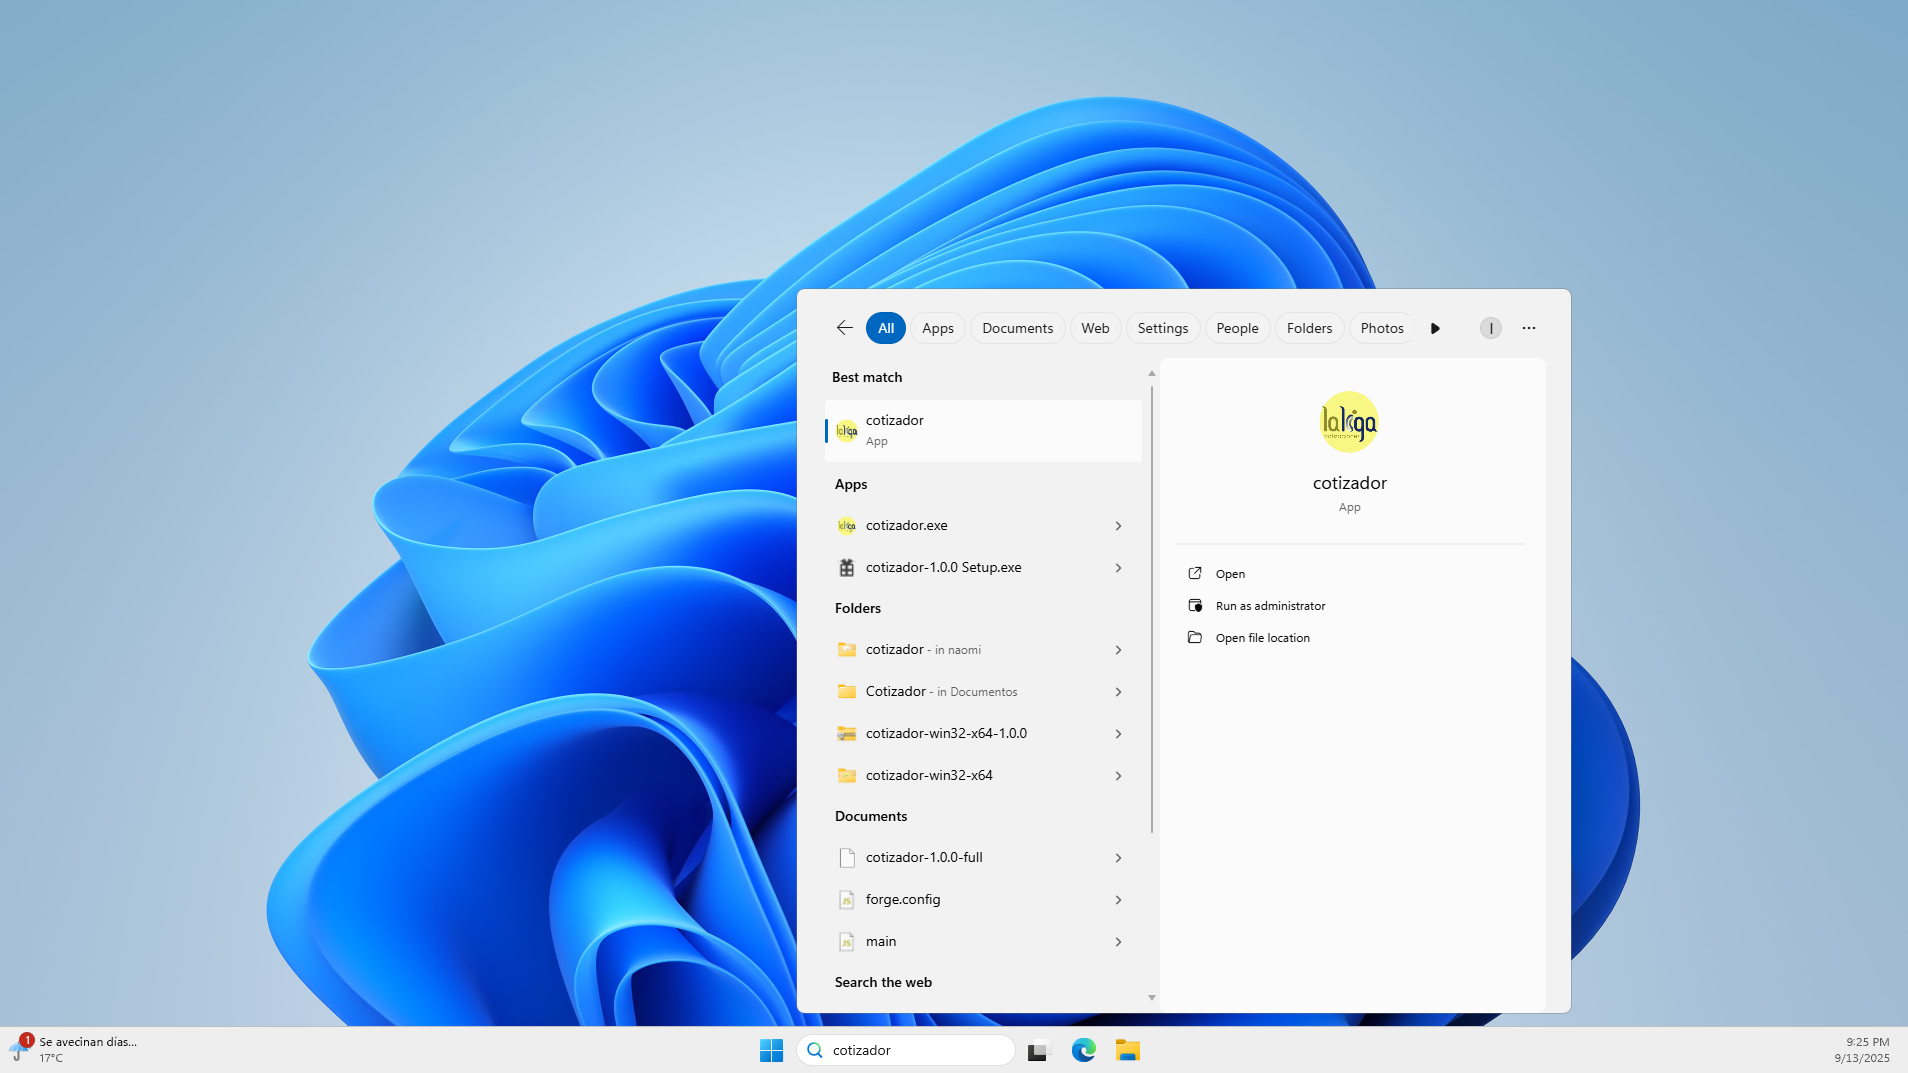
\includegraphics[width=0.85\linewidth]{img/barra-navegacion.png}
        \caption{Busca \textbf{Cotizador} en el menú de inicio de Windows.}
        \label{fig:abrir_desde_inicio}
    \end{figure}
%%%%%%%%%%%%%%%%%%%%%%%%%%%%%%%%%%%%%%%%%%%%%%%%%%%%
\pagebreak
\section{Interaz Principal y Funcionalidades}
\subsection{Explicación del menú de Gestión de Cotizaciones}

En el menu de getión de cotizaciones, se muestran todas las cotizaciones previamente realizadas, con opciones para editar,
 eliminar o generar el PDF de cada una.

\begin{figure}[H]
    \centering
    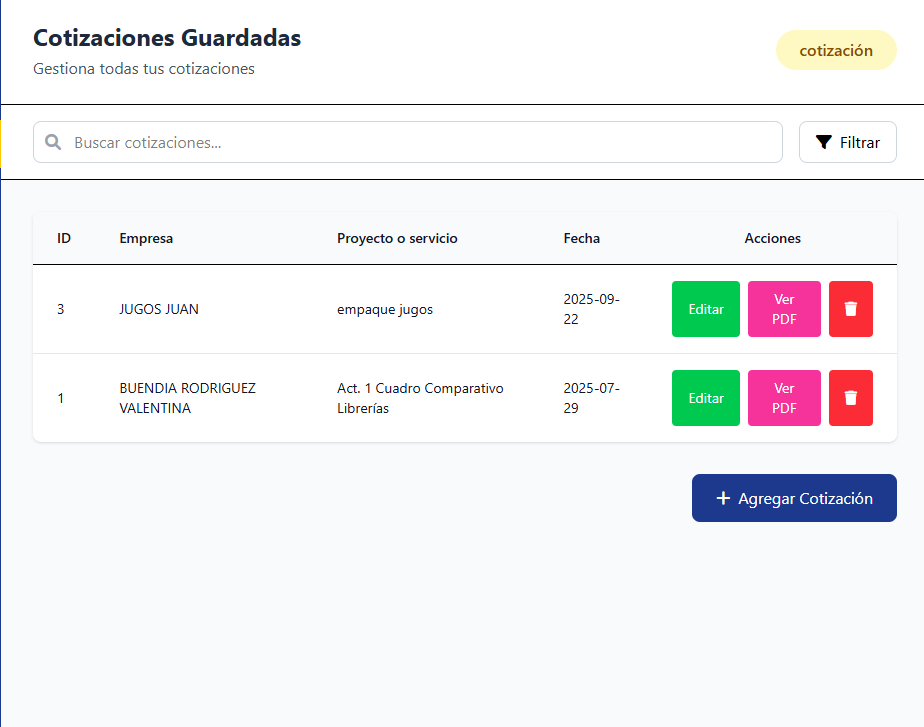
\includegraphics[width=0.8\textwidth]{img/gestion_cotizaciones.png}
    \caption{Menú de Gestión de Cotizaciones}
    \label{fig:gestion_cotizaciones}
\end{figure}

Ademas, se incluye un botón para agregar nuevas cotizaciones.

\begin{figure}[H]
    \centering
    
\includegraphics[width=0.2\textwidth]{img/agregar_cotizacion.png}
    \caption{Botón para Agregar Cotización}
    \label{fig:agregar_cotizacion}
\end{figure}

\subsection{Página para agregar cotizaciones}

En la pagina para agregar cotizaciones, se encuentran varios campos para ingresar los datos necesarios, 
como el nombre del cliente, la fecha, los productos o servicios a cotizar, y cualquier otro detalle relevante.
Ademas, se incluye un campo para importar datos desde un archivo Excel, para ello, se debe seleccionar el archivo 
deseado y la hoja correspondiente.

\begin{figure}[H]
    \centering
    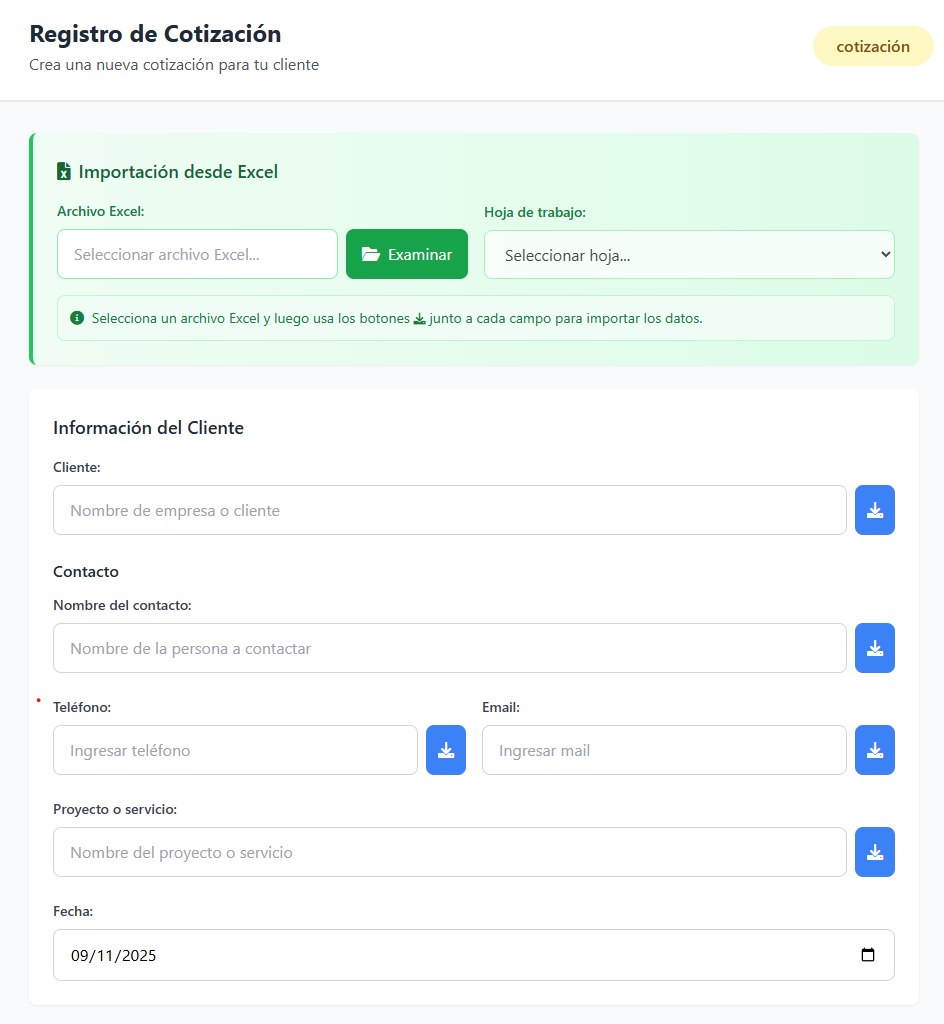
\includegraphics[width=0.8\textwidth]{img/agregar_cotizacion_pagina.png}
    \caption{Página para Agregar Cotizaciones}
    \label{fig:agregar_cotizacion_pagina}
\end{figure}

\begin{minipage}{0.68\linewidth}
    Para cada campo, hay un boton, que permite al usuario ingresar la información desde el archivo Excel seleccionado, 
    abriendo una nueva ventana con la opcion de dar click sobre la informacion deseada.
\end{minipage}
\hfil   
\begin{minipage}{0.18\linewidth}
    \begin{figure}[H]
        \centering
        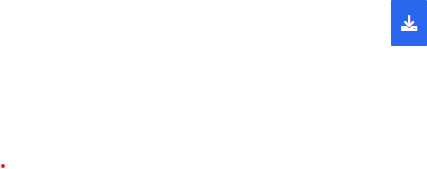
\includegraphics[width=0.6\textwidth]{img/boton_importacion.png}
        \caption{}
        \label{fig:importar_datos}
    \end{figure}
\end{minipage}


\begin{figure}[H]
    \centering
    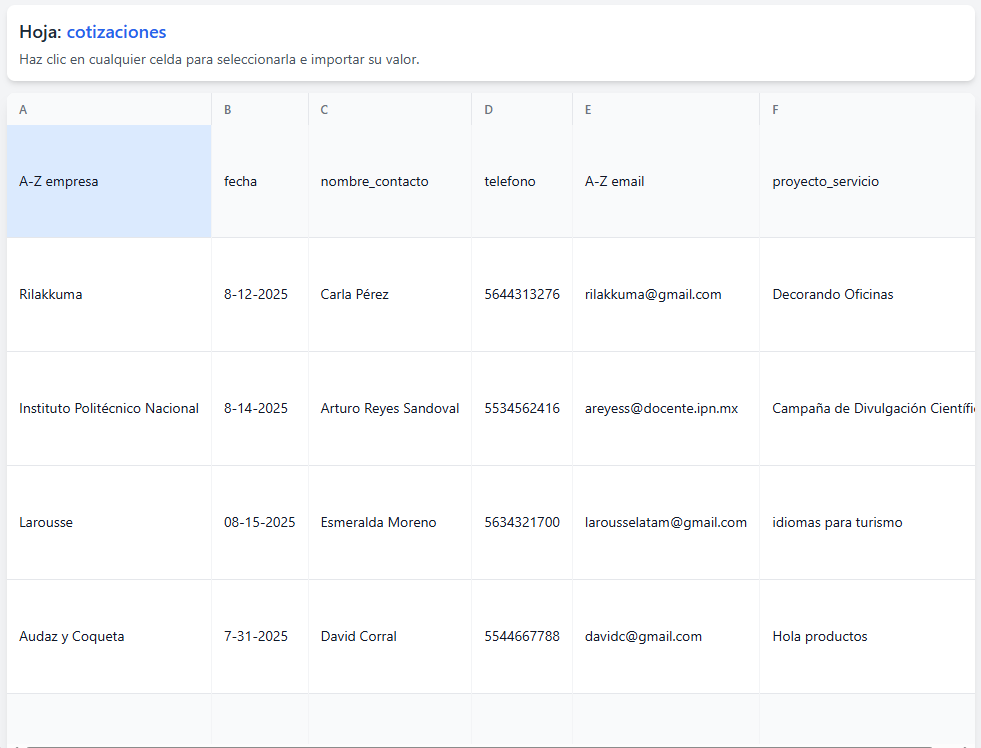
\includegraphics[width=0.6\textwidth]{img/ventana_importacion.png}
    \caption{Ventana de importación de datos}
    \label{fig:ventana_importacion}
\end{figure}


\subsubsection{Gestión de productos/servicios}

Para agregar productos, se incluyó una tabla, donde se pueden agregar, editar o eliminar productos o servicios con campos, con las mismas opciones de importación desde Excel.

\begin{figure}[H]
    \centering
    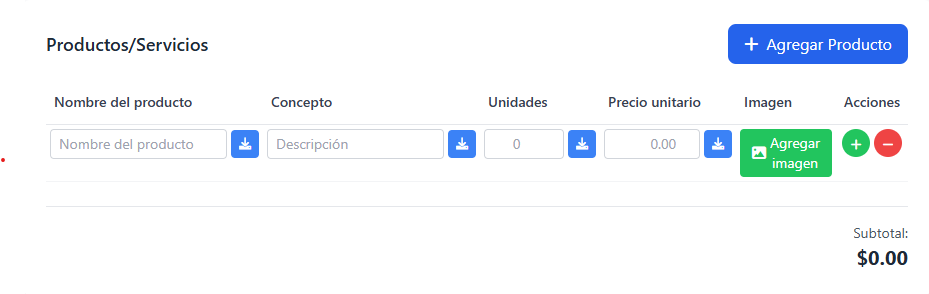
\includegraphics[width=0.8\textwidth]{img/tabla_productos.png}
    \caption{Tabla de productos/servicios}
    \label{fig:tabla_productos} 
\end{figure}

Una vez concluida la cotizacion y verificada la informacion, se puede guardar la cotizacion con el siguiente boton.

\begin{figure}[H]
    \centering
    
\includegraphics[width=0.2\textwidth]{img/boton_guardar.png}
    \caption{Botón para guardar la cotización}
    \label{fig:boton_guardar}
\end{figure}

\subsubsection{Opciones de guardado}
La aplicación cuenta con dos opciones para guardar la cotización, Guardar Cotización y Guardar borrador.
Ambas opciones guardan la cotización en la base de datos, y para cualquiera de las dos opciones, será necesario
llenar todos los campos obligatorios, de lo contrario, se mostrará un mensaje de error. 
\begin{figure}[H]
    \centering
    
\includegraphics[width=0.4\textwidth]{img/opciones_guardado.png}
    \caption{Botones de las dos opciones de guardado}
    \label{fig:opciones_guardado}
\end{figure}
Los campos obligatorios son 
los datos personales del cliente, la fecha, el nombre del producto/servicio, y la información de contacto.\\
 Si al registrar la cotización no cuentas con alguno de estos datos, la recomendación
 es poner algún dato temporal y editarlo después.
\begin{figure}[H] 
    \centering
        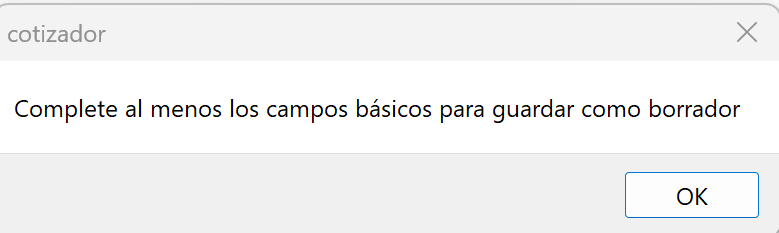
\includegraphics[width=0.35\linewidth]{img/mensaje_error.png}
    \caption{Si no se llenan los campos obligatorios, se mostrará este mensaje de error y la cotización no se guardará.}
    \label{fig:mensaje_error}
\end{figure}

%%%%%%%%%%%%%%%%%%%%%%%%%%%%%%%%%%%%%%%%%%%%%%%%%%%%
\section{Ejemplos prácticos}
\subsection{Cómo registrar una cotización}
Al abrir por primera vez la aplicación, la página de \textbf{Cotizaciones guardadas} se verá como se muestra en la figura~\ref{fig:vista_inicial}.
Como aun no hay registros de cotizaciones, la tabla estará vacía. 
    \begin{figure}[H]
        \centering
            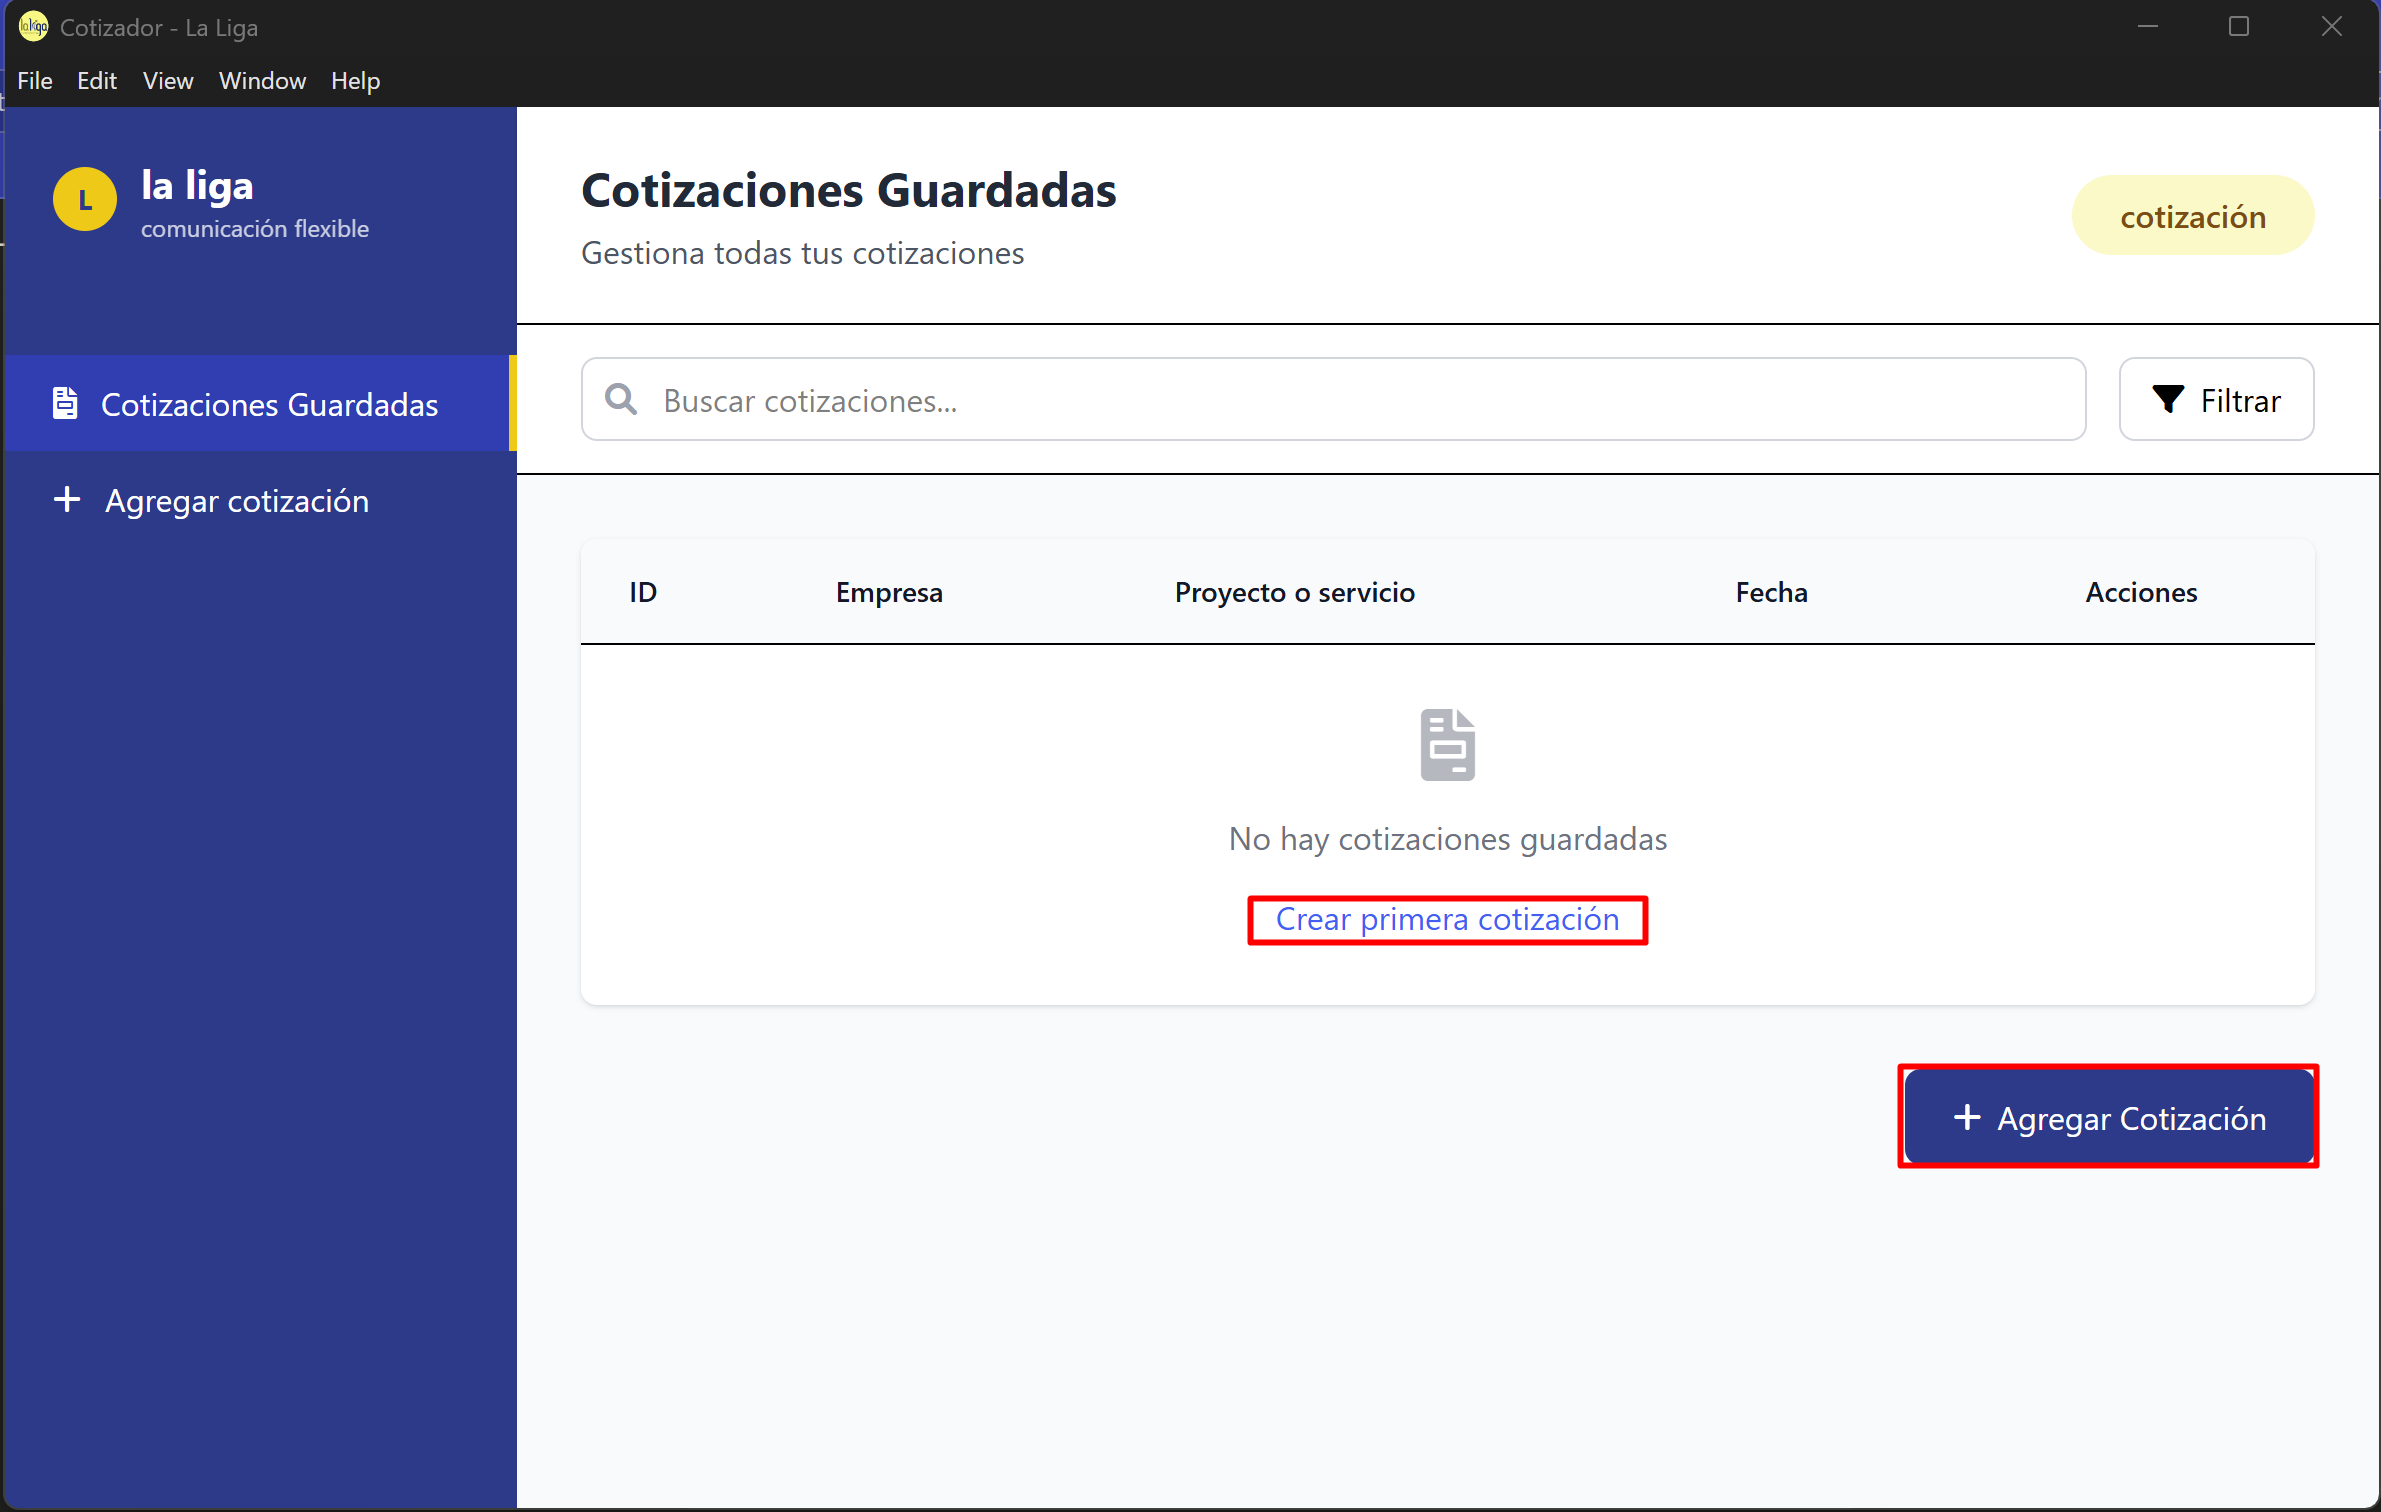
\includegraphics[width=0.85\linewidth]{img/abrir_primera_vez.png}
        \caption{Vista inicial de la página de cotizaciones guardadas al abrir la aplicación por primera vez.}
        \label{fig:vista_inicial}
    \end{figure}
Para agregar una nueva cotización, haz clic en el botón \textbf{Agregar Cotización} o dentro de
la tabla en \textbf{Crear primera cotización}. Esto te llevará a la página para agregar una nueva cotización, donde podrás ingresar los 
detalles necesarios de la cotización.

\begin{figure}[H] 
    \centering
        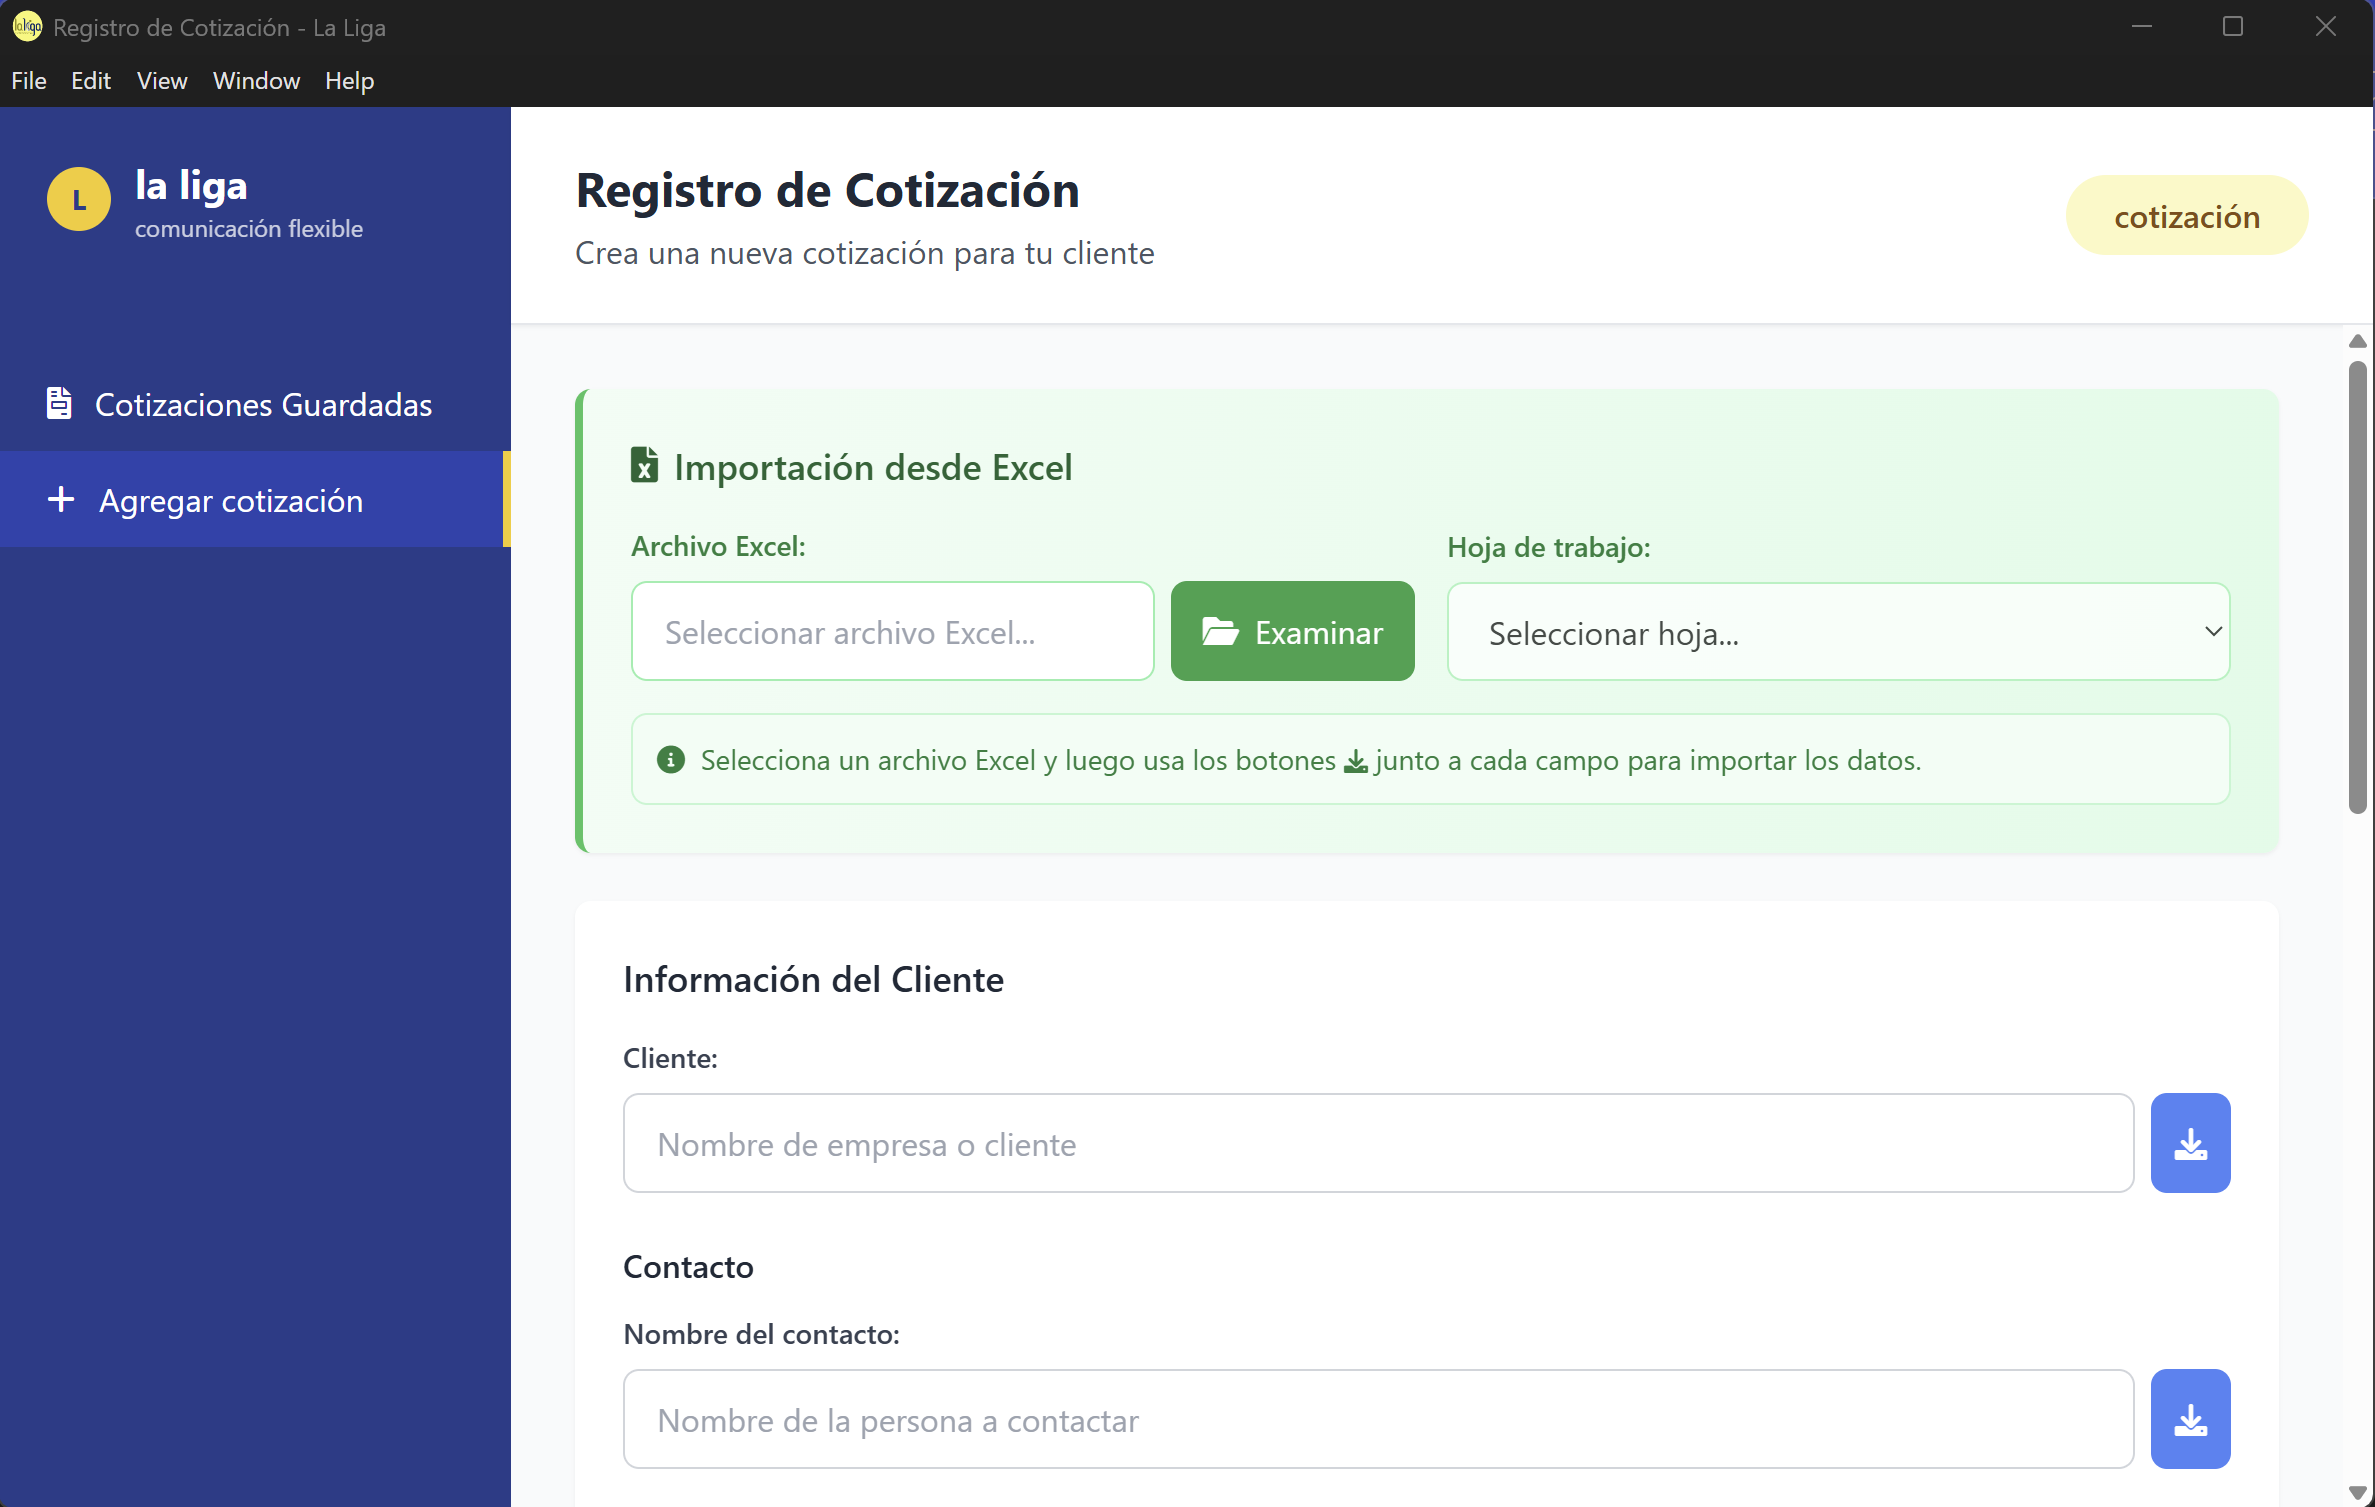
\includegraphics[width=0.8\linewidth]{img/add_cotizacion_inicial.png}
\caption{Vista inicial de la página de agregar cotización al abrir la aplicación por primera vez.}\label{fig:vista_inicial_add}
\end{figure}
En esta parte podrás elegir entre dos opciones para ingresar los datos, la primera es dando clic sobre los campos y escribir a través del teclado.
\begin{figure}[H] 
    \centering
        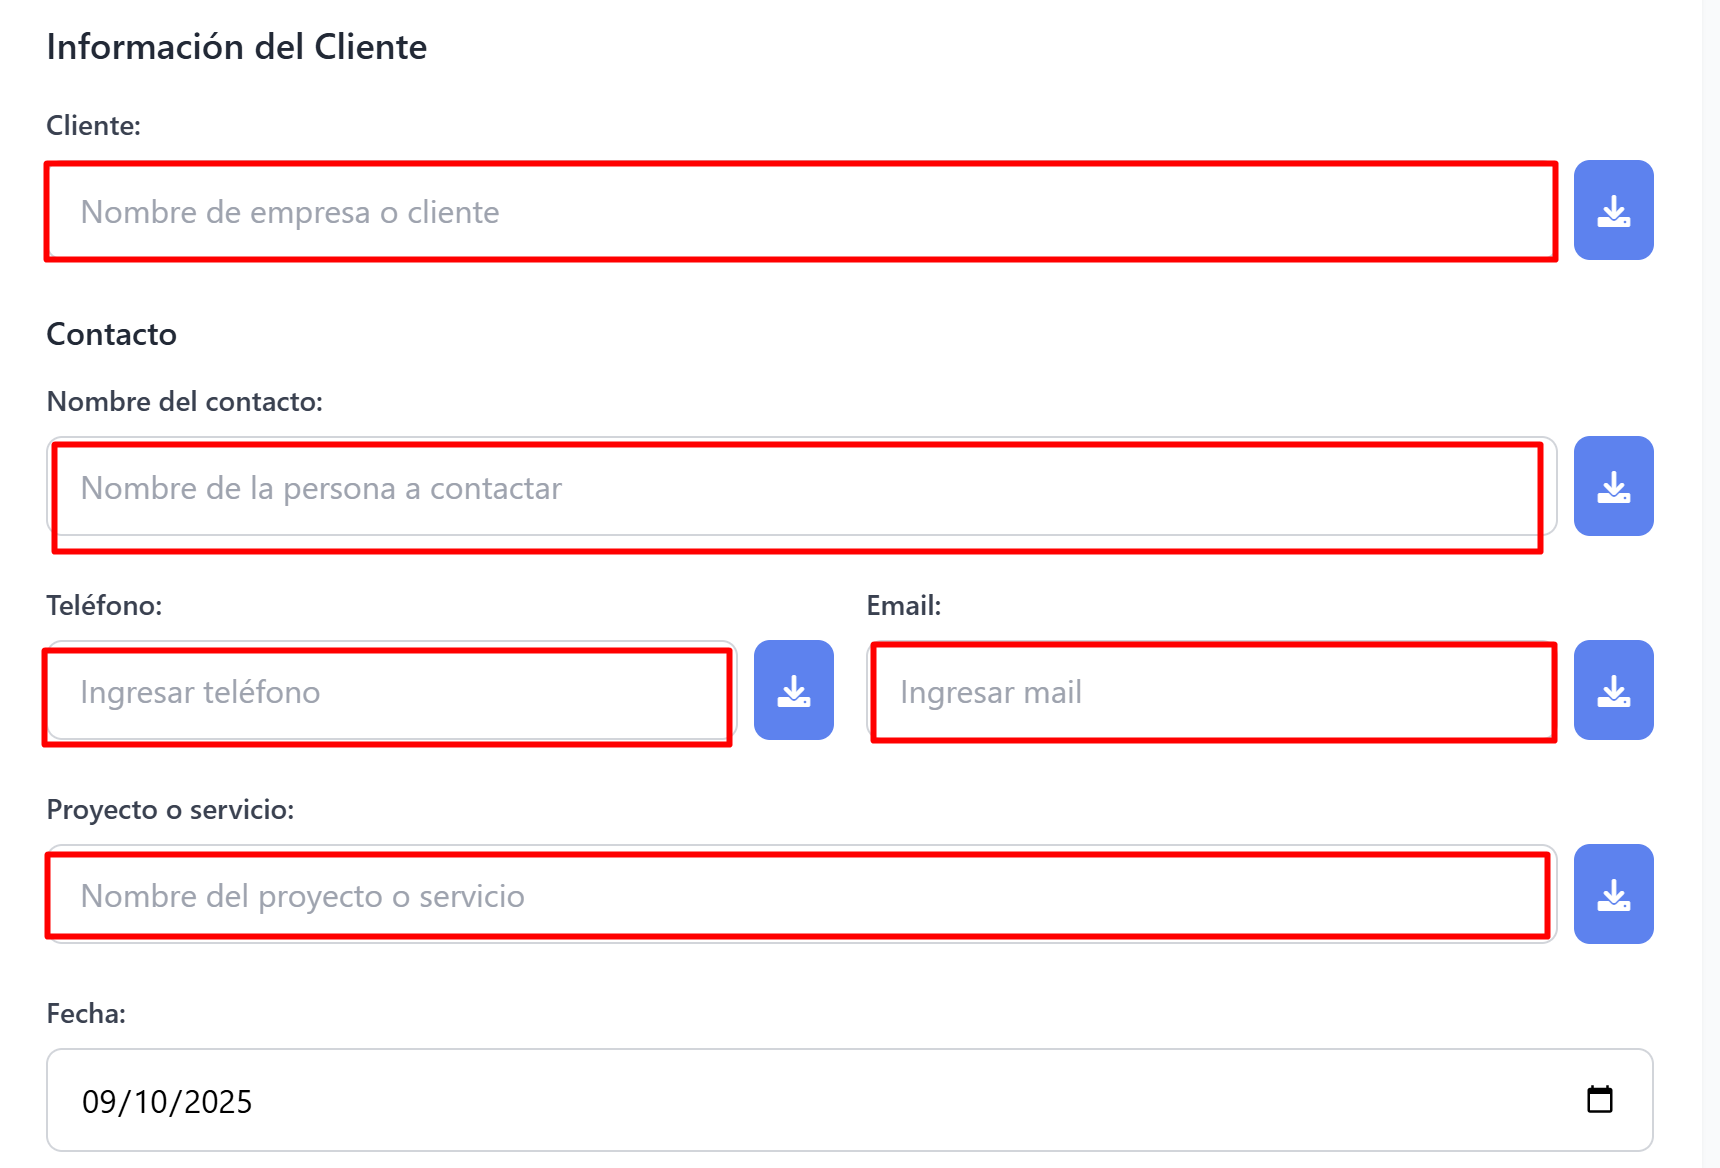
\includegraphics[width=0.7\linewidth]{img/llenar_campos.png}
    \caption{Da clic en los campos y escribe para llenarlos manualmente.}
    \label{fig:llenado_manual1}
\end{figure}
La segunda opción es importando los datos desde un archivo de Excel. Para ello, dirígete a la sección de 
\textbf{Importación desde Excel} que encontrarás hasta arriba de la ventana y haz clic en el botón \textbf{Examinar}. A continuación, se abrirá una ventana 
del Explorador de archivos donde podrás seleccionar el archivo de Excel que contiene los datos de la cotización que deseas importar. Asegúrate de que el archivo 
esté en formato .xlsx o .xls.\\
Si el archivo se carga correctamente, verás el nombre del archivo en el área debajo del botón \textbf{Examinar}, 
como se muestra en la figura~\ref{fig:archivos_cargados}.
\begin{figure}[H] 
    \centering
        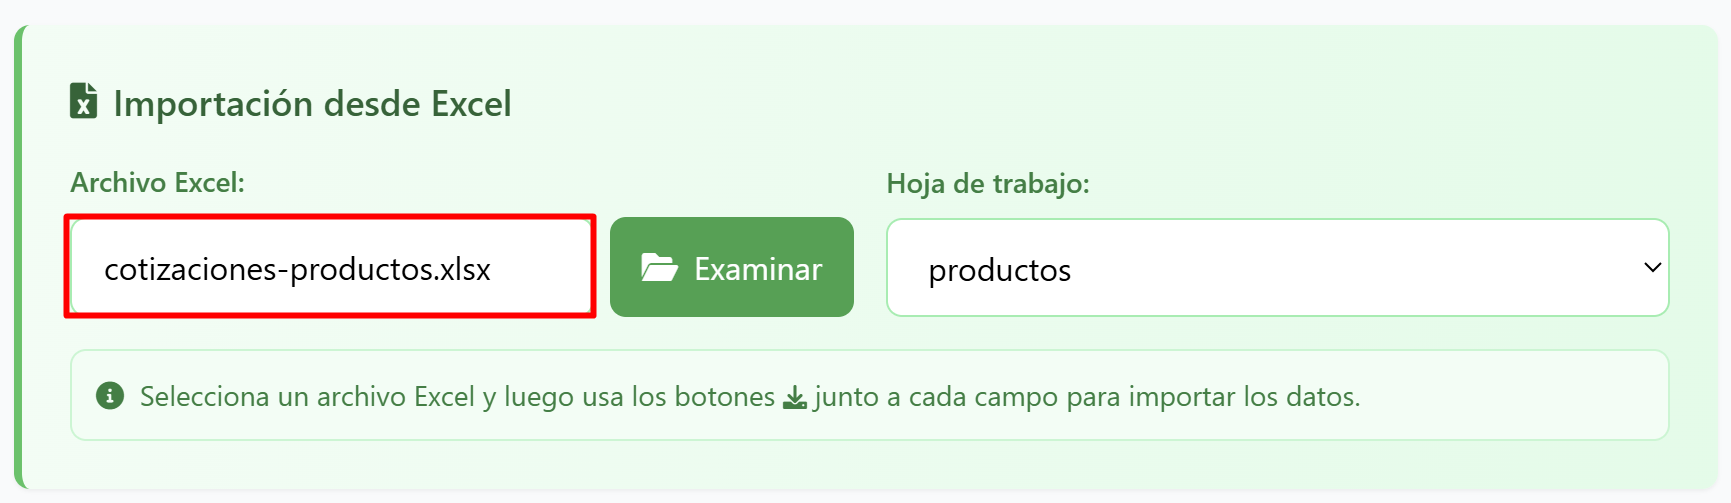
\includegraphics[width=0.7\linewidth]{img/archivos_cargados.png}
    \caption{Una vez que seleccionaste el archivo desde tu almacenamiento, verás el nombre del archivo en esta área.}
    \label{fig:archivos_cargados}
\end{figure}
Lo que deberás hacer a continuación es seleccionar la hoja del archivo de Excel que contiene los datos que deseas importar. 
Para ello, haz clic en el menú desplegable que se encuentra abajo del texto  \textbf{Hoja de trabajo} y elige la hoja correspondiente.
\begin{figure}[H] 
    \centering
        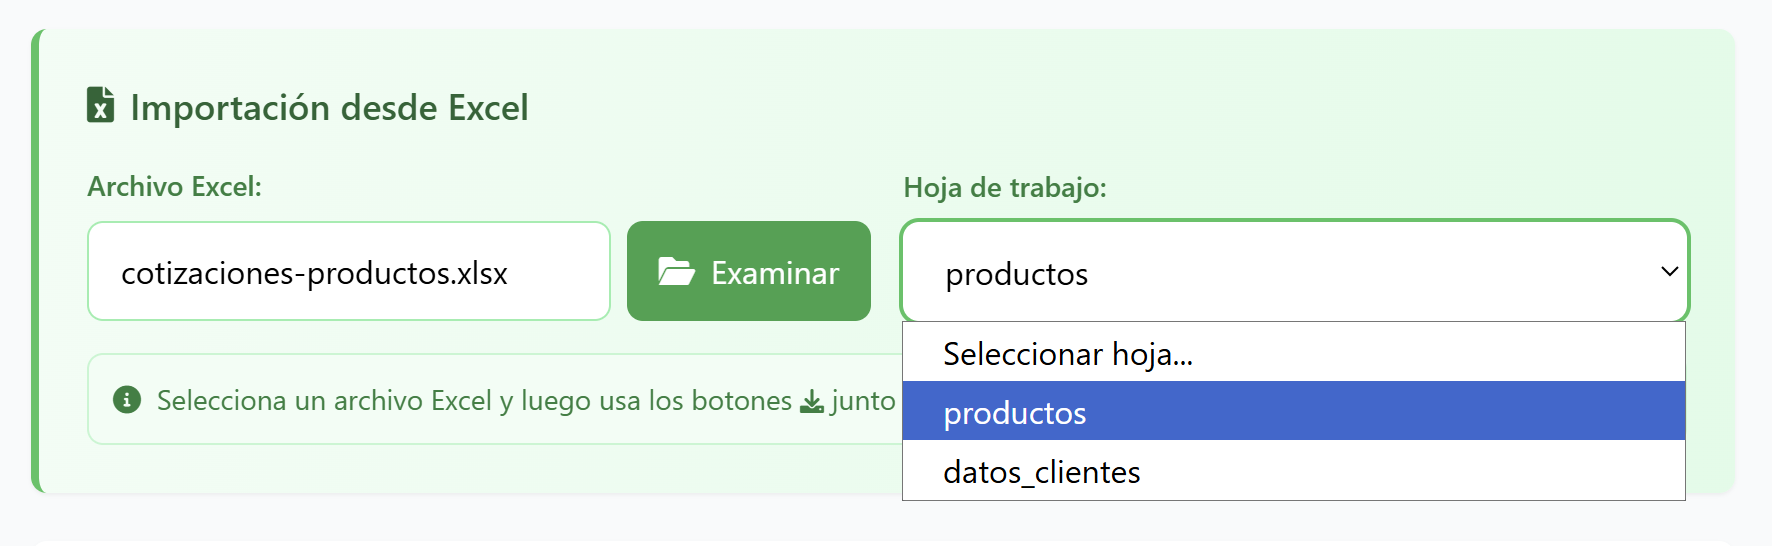
\includegraphics[width=0.7\linewidth]{img/seleccionar_hoja.png}
    \caption{Selecciona la hoja del archivo de Excel que contiene los datos que deseas importar.}
    \label{fig:seleccionar_hoja}
\end{figure}

Una vez que hayas seleccionado la hoja, podrás comenzar a importar los datos a los campos correspondientes.
En cada campo, verás un botón con un ícono en color azul (figura \ref{fig:importar_datos}), al seleccionarlo
 se abrirá una ventana emergente que mostrará los datos de la hoja de Excel seleccionada.
 
\begin{figure}[H]
    \centering
    \begin{minipage}{0.456\linewidth}
        \centering
        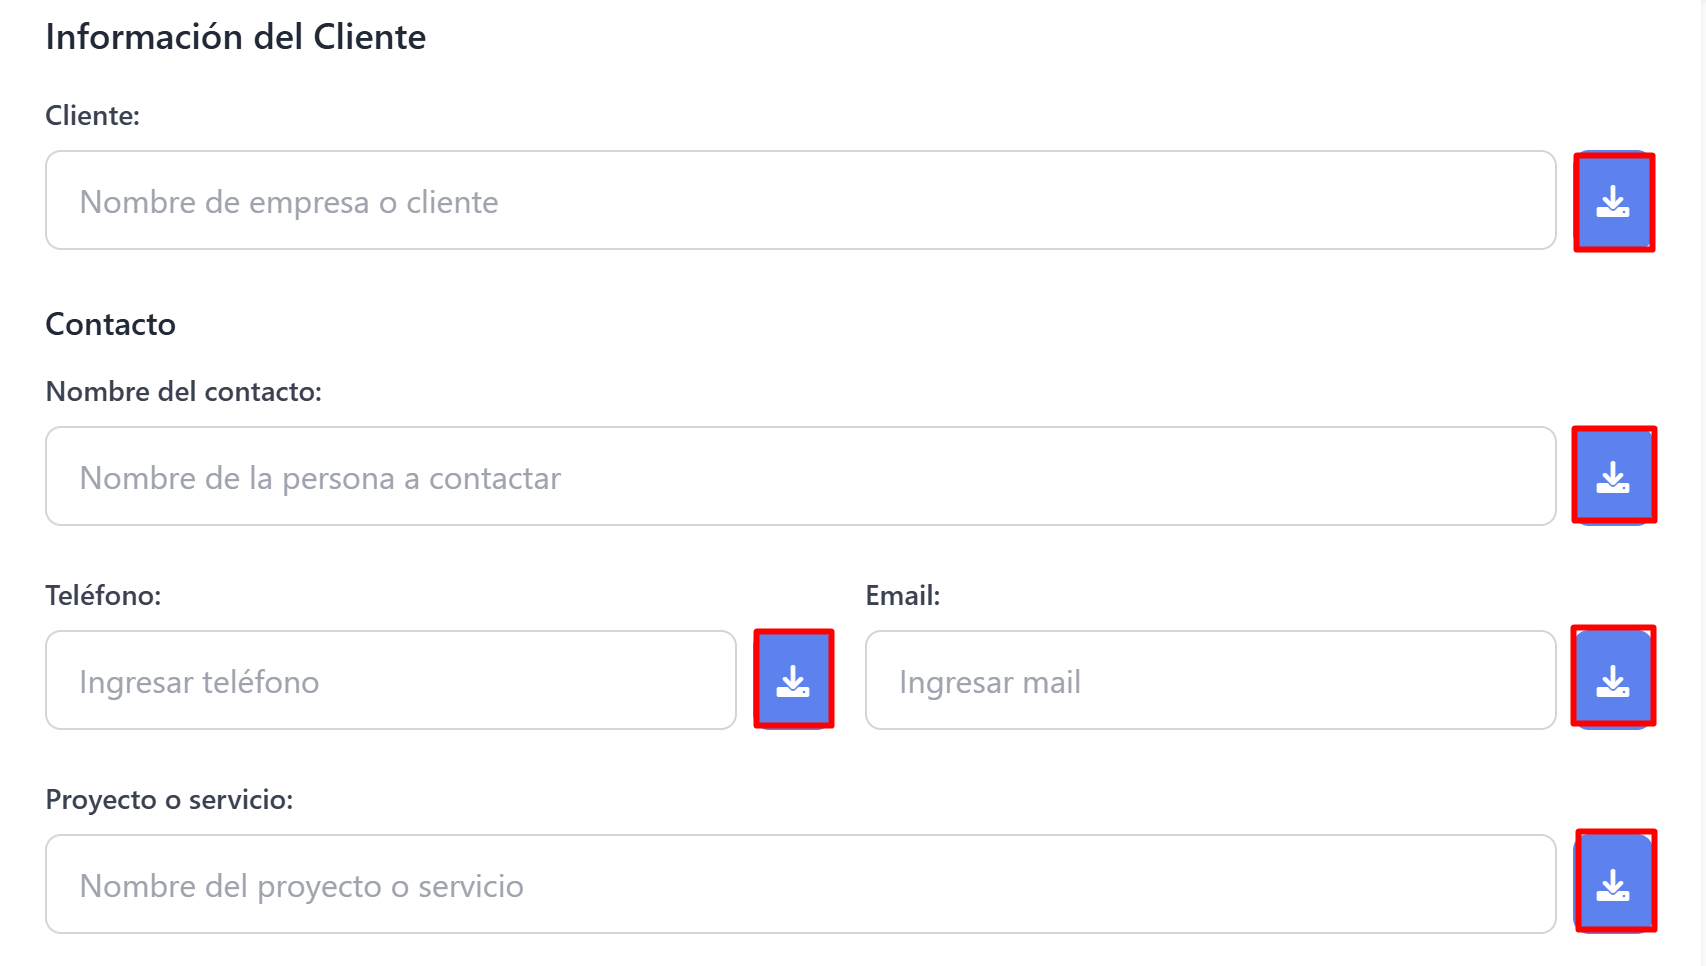
\includegraphics[width=\linewidth]{img/llenar_datos_excel.png}
    \end{minipage}
    \begin{minipage}{0.49\linewidth}
        \centering
        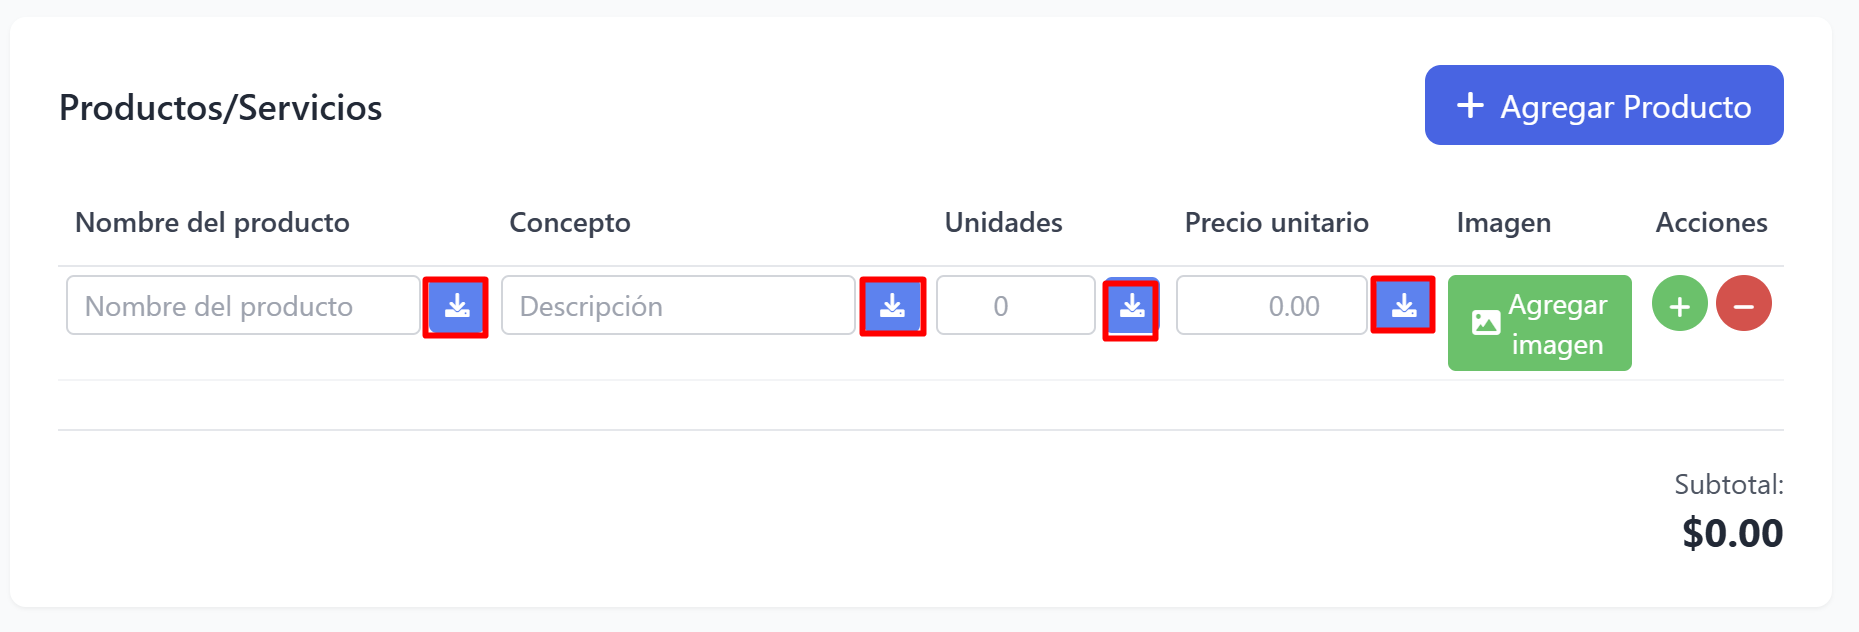
\includegraphics[width=\linewidth]{img/registrar_productos_excel.png}
    \end{minipage}

    \caption{Icono para importar datos desde Excel}
    \label{fig:icono-importar}
\end{figure}

La ventana emergente mostrará una tabla con los datos de la hoja de Excel seleccionada.
Para importar un dato específico a un campo, simplemente haz clic en la celda correspondiente en la tabla.
\begin{figure}[H] 
    \centering
        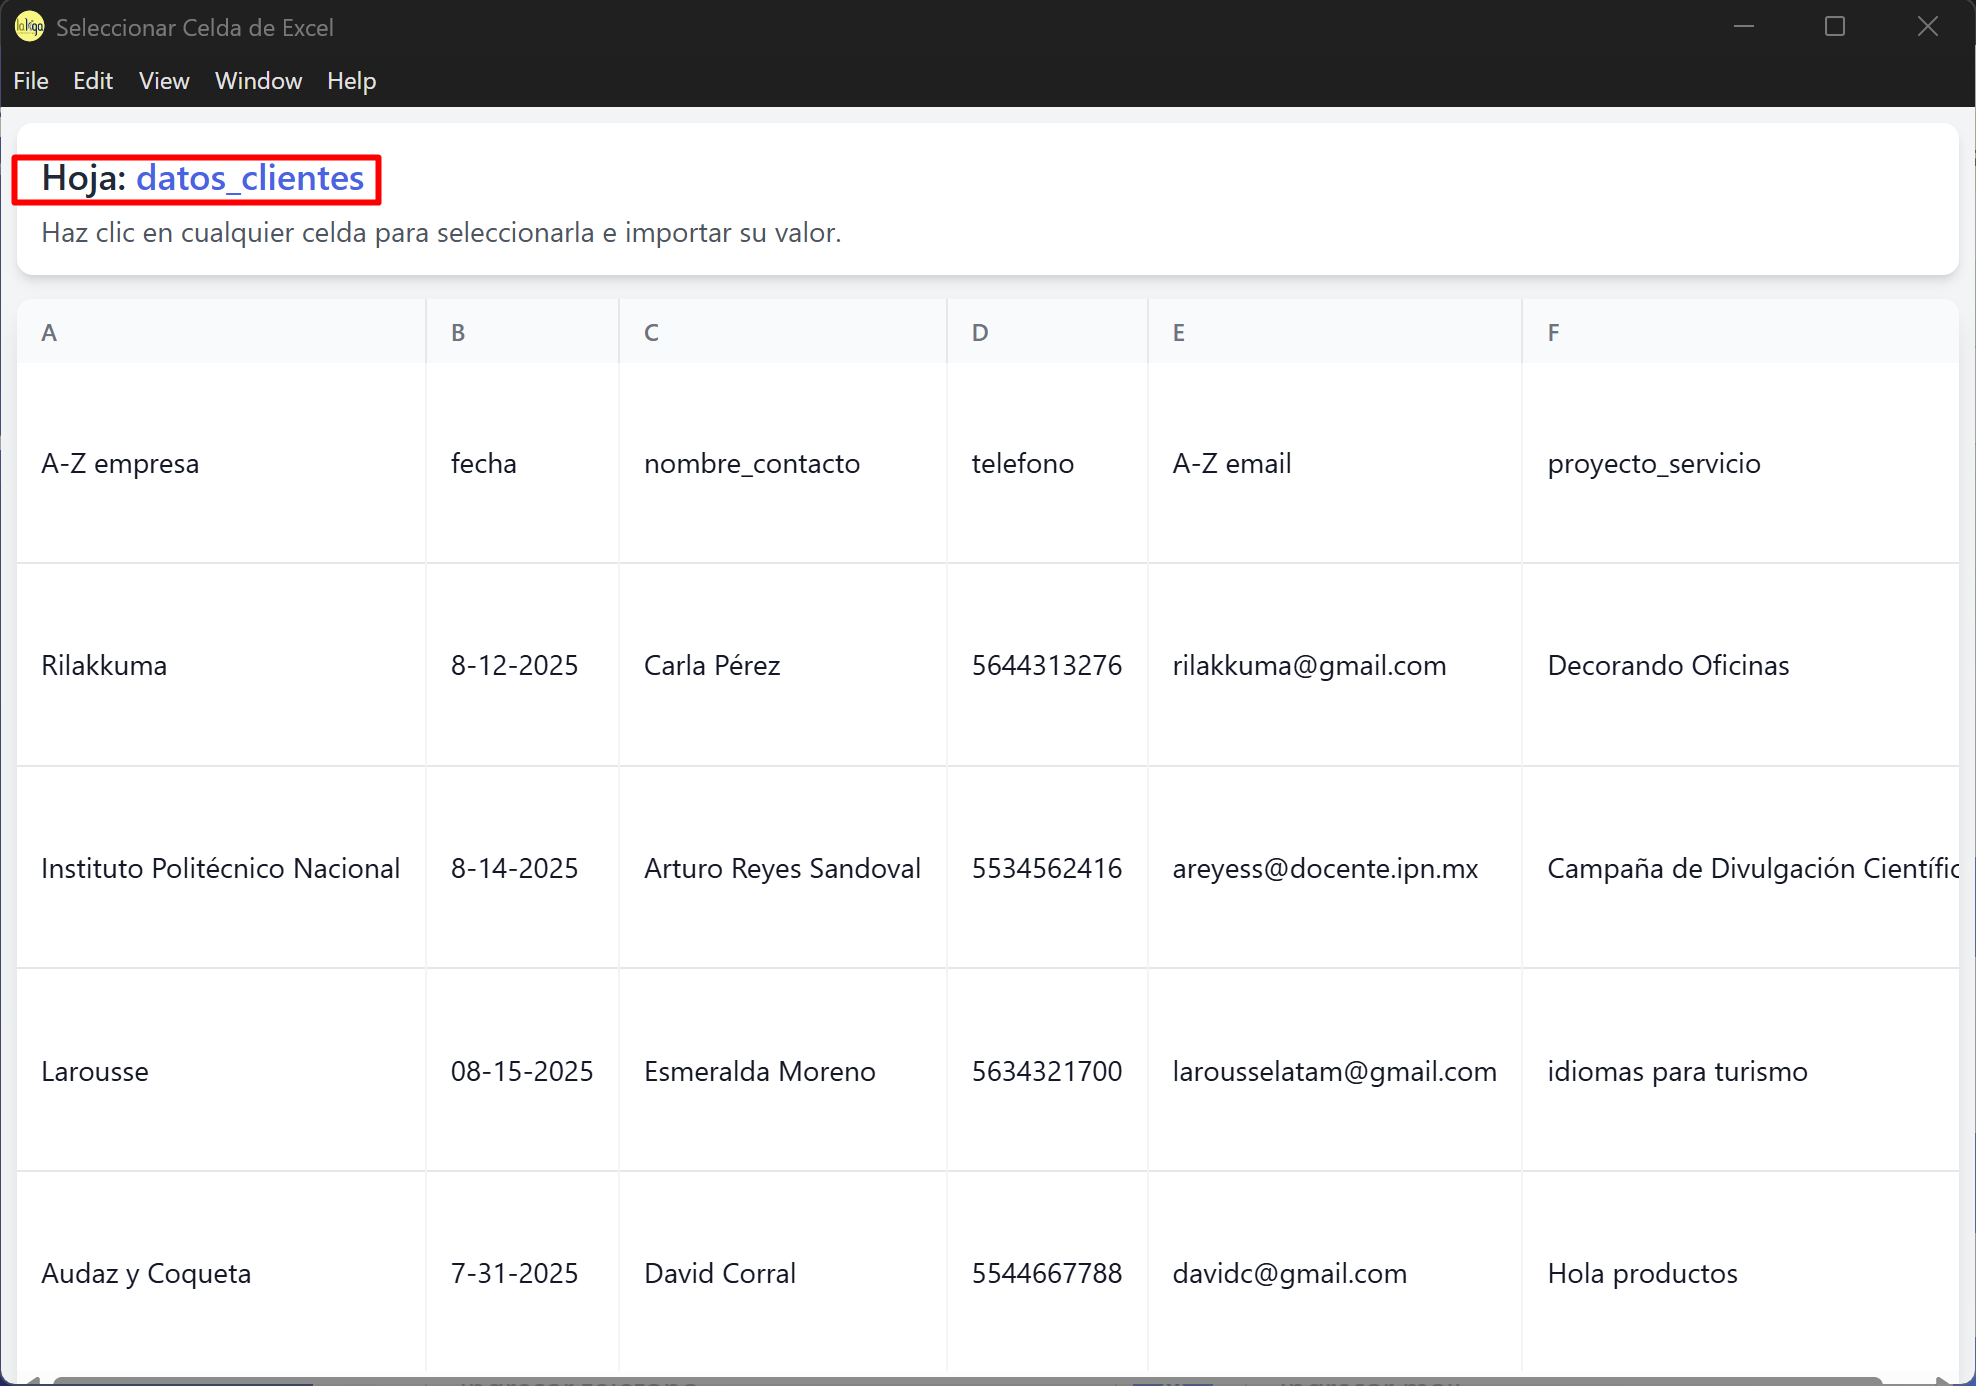
\includegraphics[width=0.6\linewidth]{img/hoja_excel.png}
    \caption{Ventana emergente para seleccionar datos desde la hoja de Excel.}
    \label{fig:seleccionar_hoja}
\end{figure}

Una vez que hayas seleccionado el dato, la ventana emergente se cerrará automáticamente y el campo se llenará 
con el valor seleccionado. Repite este proceso para cada campo que desees llenar desde el archivo de Excel.
\\\\
Cuando hayas terminado de llenar todos los campos necesarios, ya sea manualmente o mediante la importación desde Excel,
puedes proceder a guardar la cotización. Para ello, selecciona \textbf{Guardar Cotización} o \textbf{Guardar Borrador}.
 Si todos los campos obligatorios están completos, la cotización se 
guardará correctamente y serás redirigido de vuelta a la página de \textbf{Cotizaciones guardadas}.

\subsubsection{Cómo agregar productos a una cotización}
Para agregar productos o servicios a la cotización, dirígete a la sección de \textbf{Productos/Servicios} que se encuentra 
en la parte inferior de la página de agregar cotización.
\begin{figure}[H] 
    \centering
        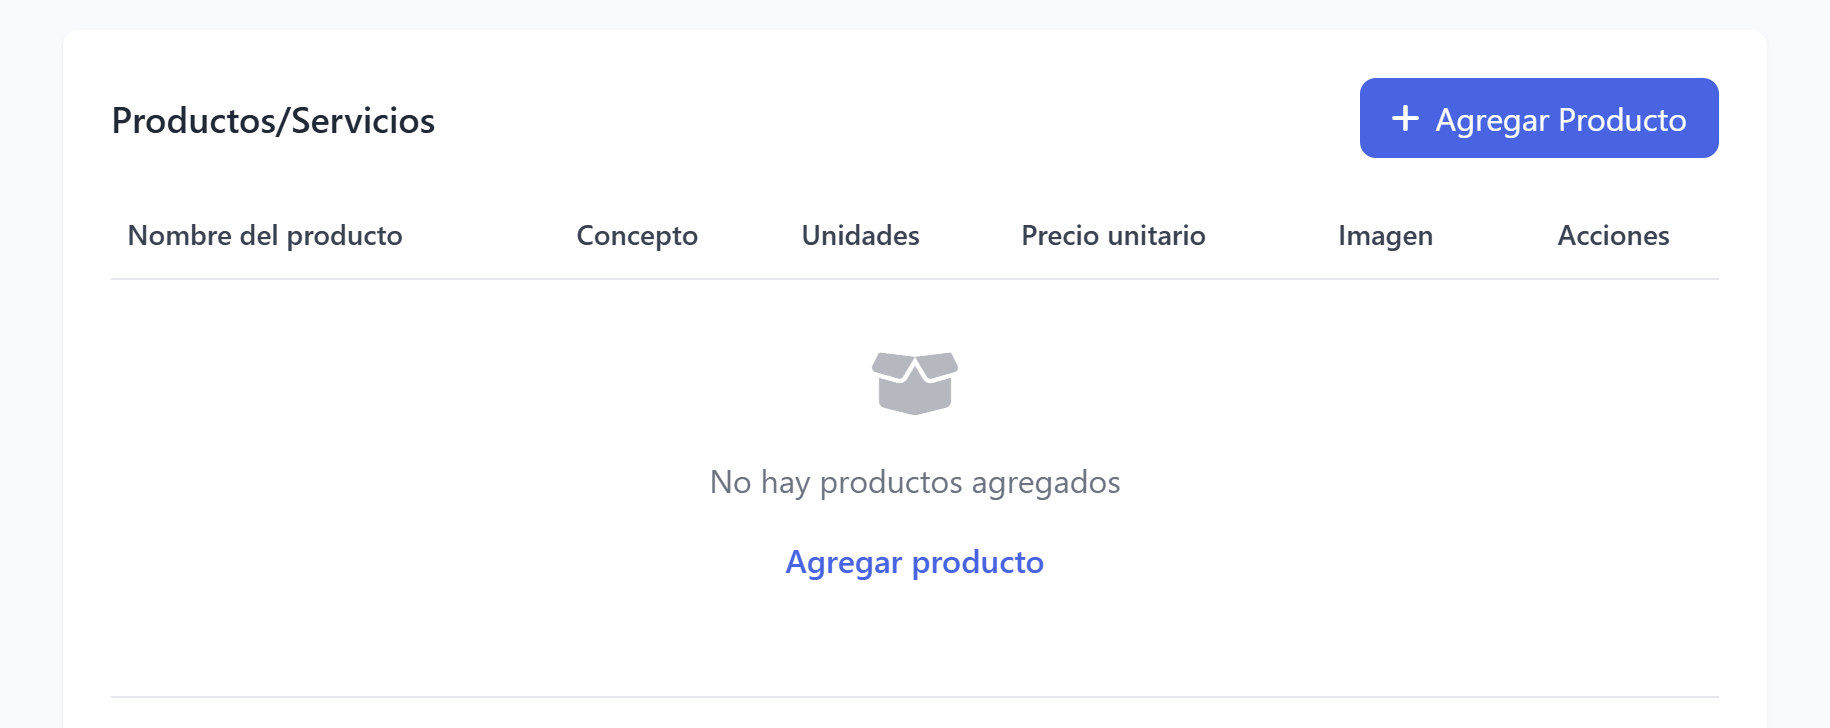
\includegraphics[width=0.75\linewidth]{img/seccion_productos.png}
    \caption{Sección de Productos/Servicios en la página de agregar cotización.}
    \label{fig:seccion_productos}
\end{figure}
En esta sección, verás una tabla con los siguientes campos: \textbf{Nombre del producto/servicio}, \textbf{Concepto}, \textbf{Unidades}, 
\textbf{Precio unitario} e \textbf{Imagen}.
Para agregar un nuevo producto o servicio por primera vez, haz clic en el botón \textbf{Agregar Producto} que se encuentra arriba 
de la tabla, o bien dentro de la tabla, como se muestra en la figura~\ref{fig:seccion_productos}.

Aparecerá una nueva fila en la tabla con campos vacíos donde podrás ingresar los detalles del producto o servicio.

\begin{figure}[H] 
    \centering
        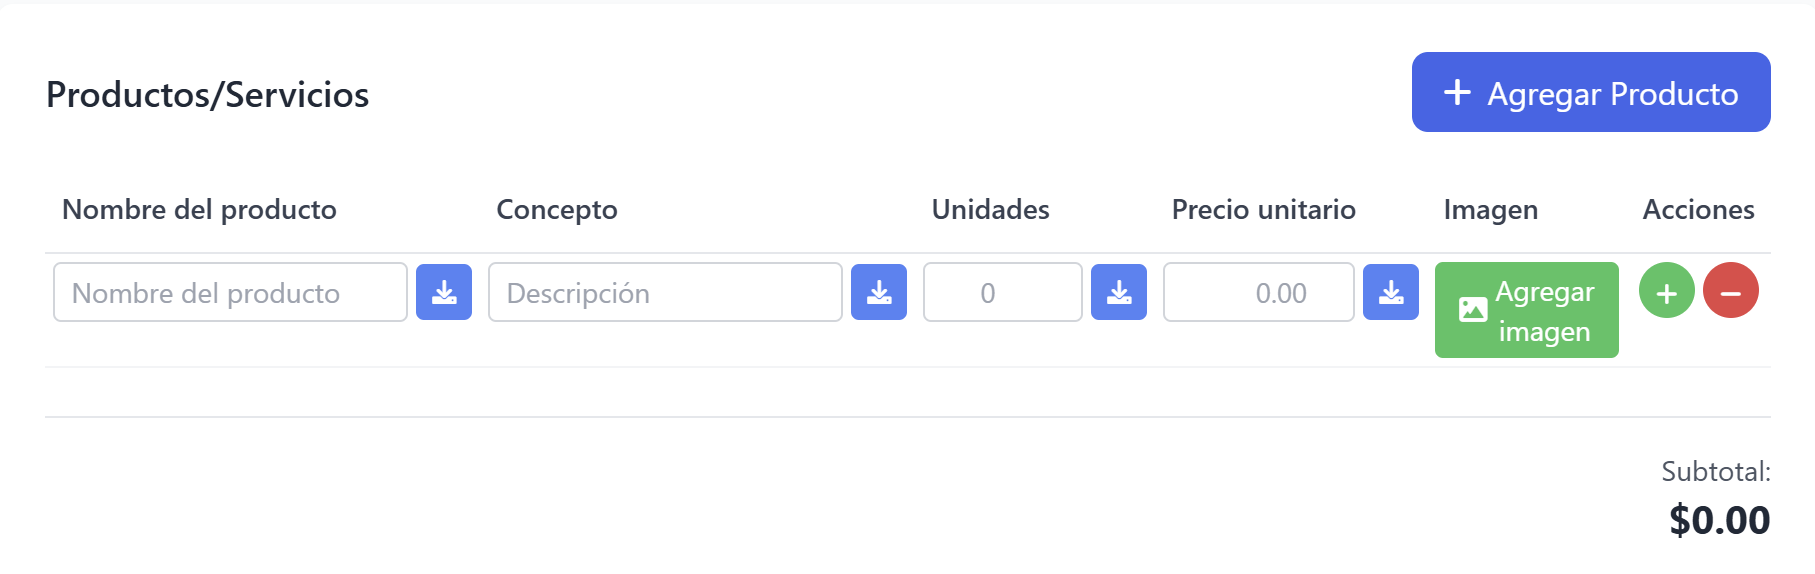
\includegraphics[width=0.8\linewidth]{img/agregar_producto.png}
    \caption{Fila vacía tras dar clic en \textbf{Agregar Producto}.}
    \label{fig:llenar_producto}
\end{figure}
Para llenar los campos correspondientes con la información del producto o servicio, puedes hacerlo ingresando
los datos manualmente o importándolos desde un archivo de Excel, siguiendo el mismo procedimiento descrito anteriormente.
\begin{figure}[H] 
    \centering
        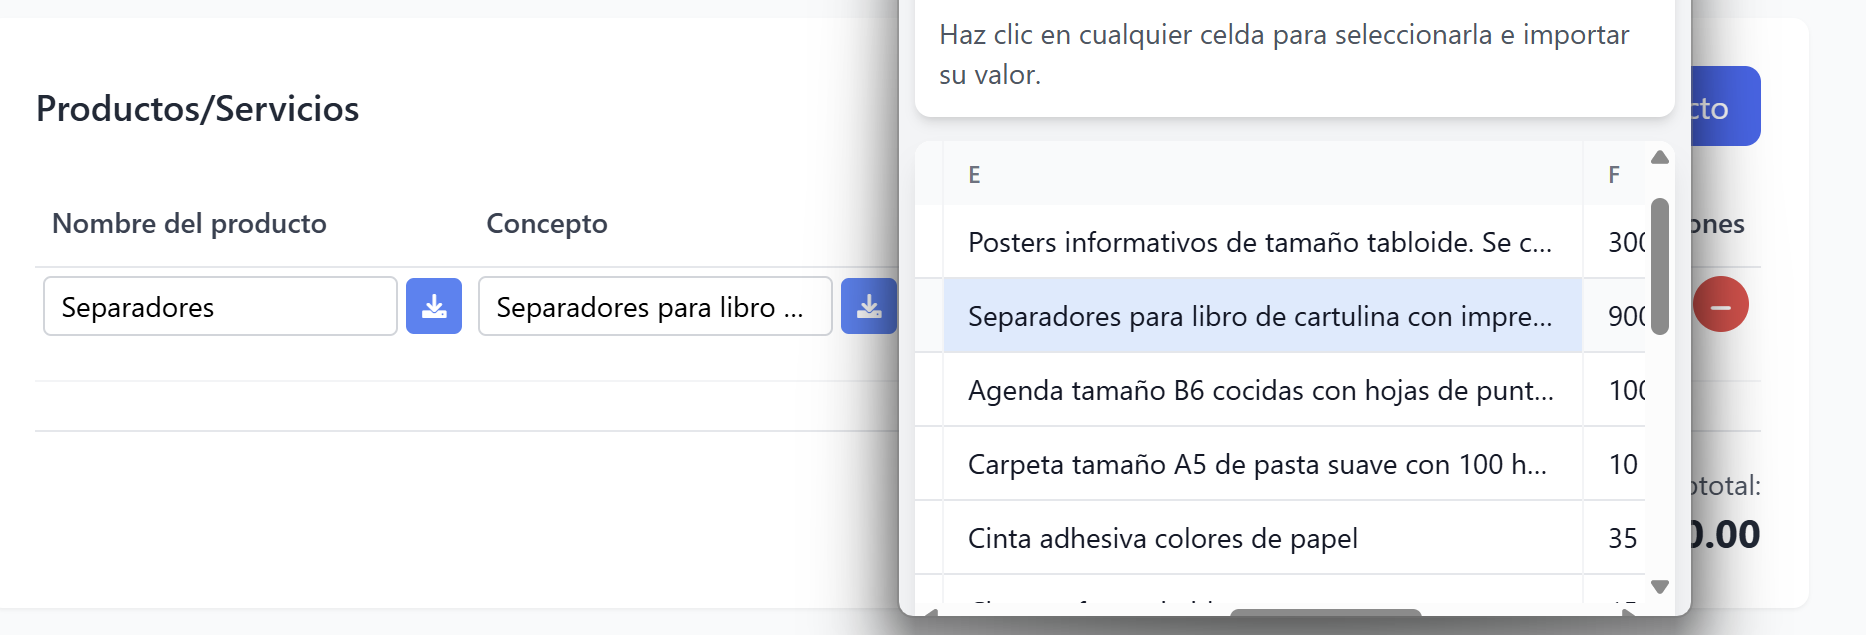
\includegraphics[width=0.8\linewidth]{img/concepto.png}
    \caption{Llena los campos con la información del producto o servicio.}
    \label{fig:llenar_producto}
\end{figure}
En el campo de Concepto, puedes ingresar una descripción detallada del producto o servicio, incluyendo características, beneficios o 
cualquier otra información relevante que ayude a entender mejor lo que se está cotizando. Aunque no se muestre por completo en el campo
de la tabla, el texto completo se reflejará en el archivo pdf de la cotización.

\subsubsection{Cómo agregar una imagen a un producto/servicio}
Para agregar una imagen a un producto o servicio, dirígete a la columna \textbf{Imagen} en la fila correspondiente al producto o servicio al 
que deseas agregar la imagen. Haz clic en el botón con el ícono de una imagen que se encuentra en esa columna, como se muestra en
 la figura~\ref{fig:icono_imagen}. 
\begin{figure}[H] 
    \centering
        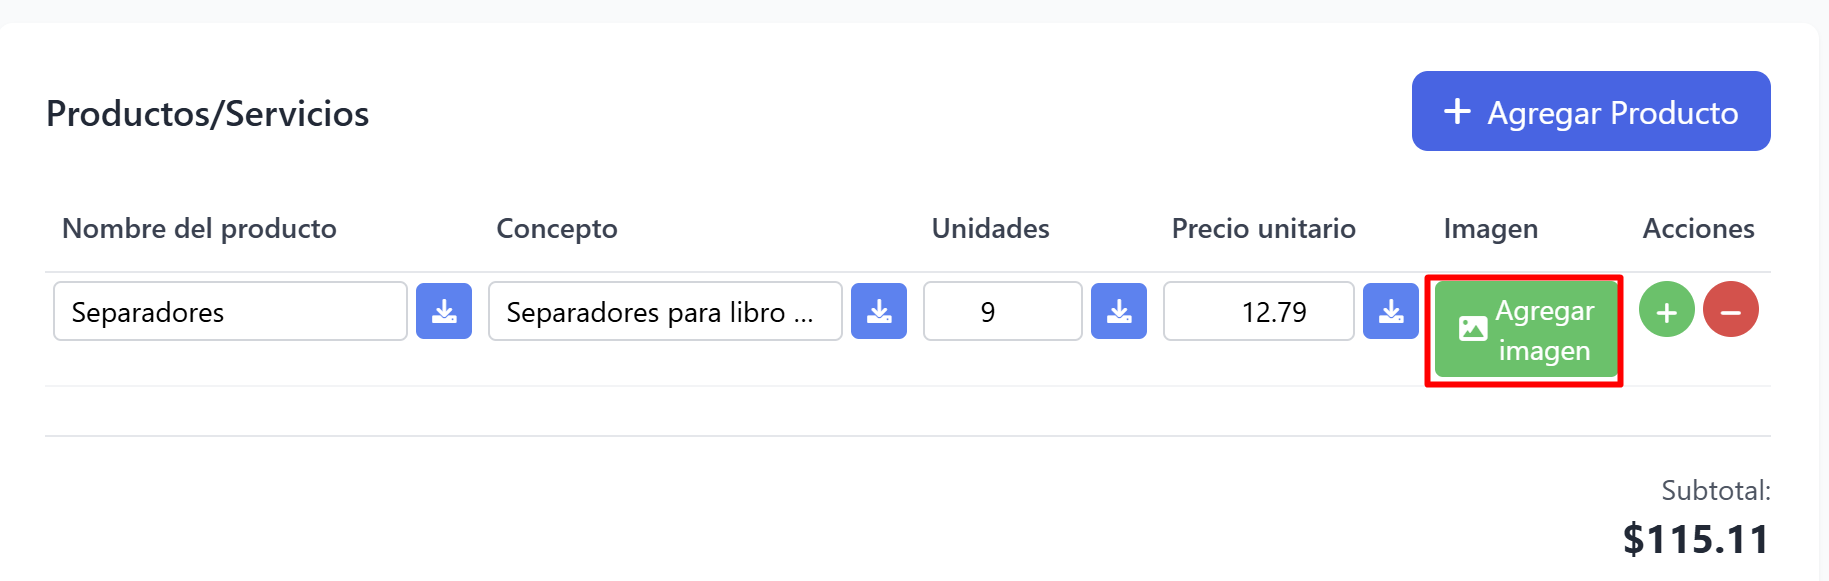
\includegraphics[width=0.8\linewidth]{img/icono_imagen.png}
    \caption{Ícono para agregar una imagen a un producto o servicio.}
    \label{fig:icono_imagen}
\end{figure}
Se abrirá una ventana del Explorador de archivos donde podrás seleccionar la imagen que deseas agregar. Asegúrate de que la imagen esté en
formato JPEG o PNG. Una vez que selecciones la imagen, se visualizará en la tabla.
\begin{figure}[H] 
    \centering
        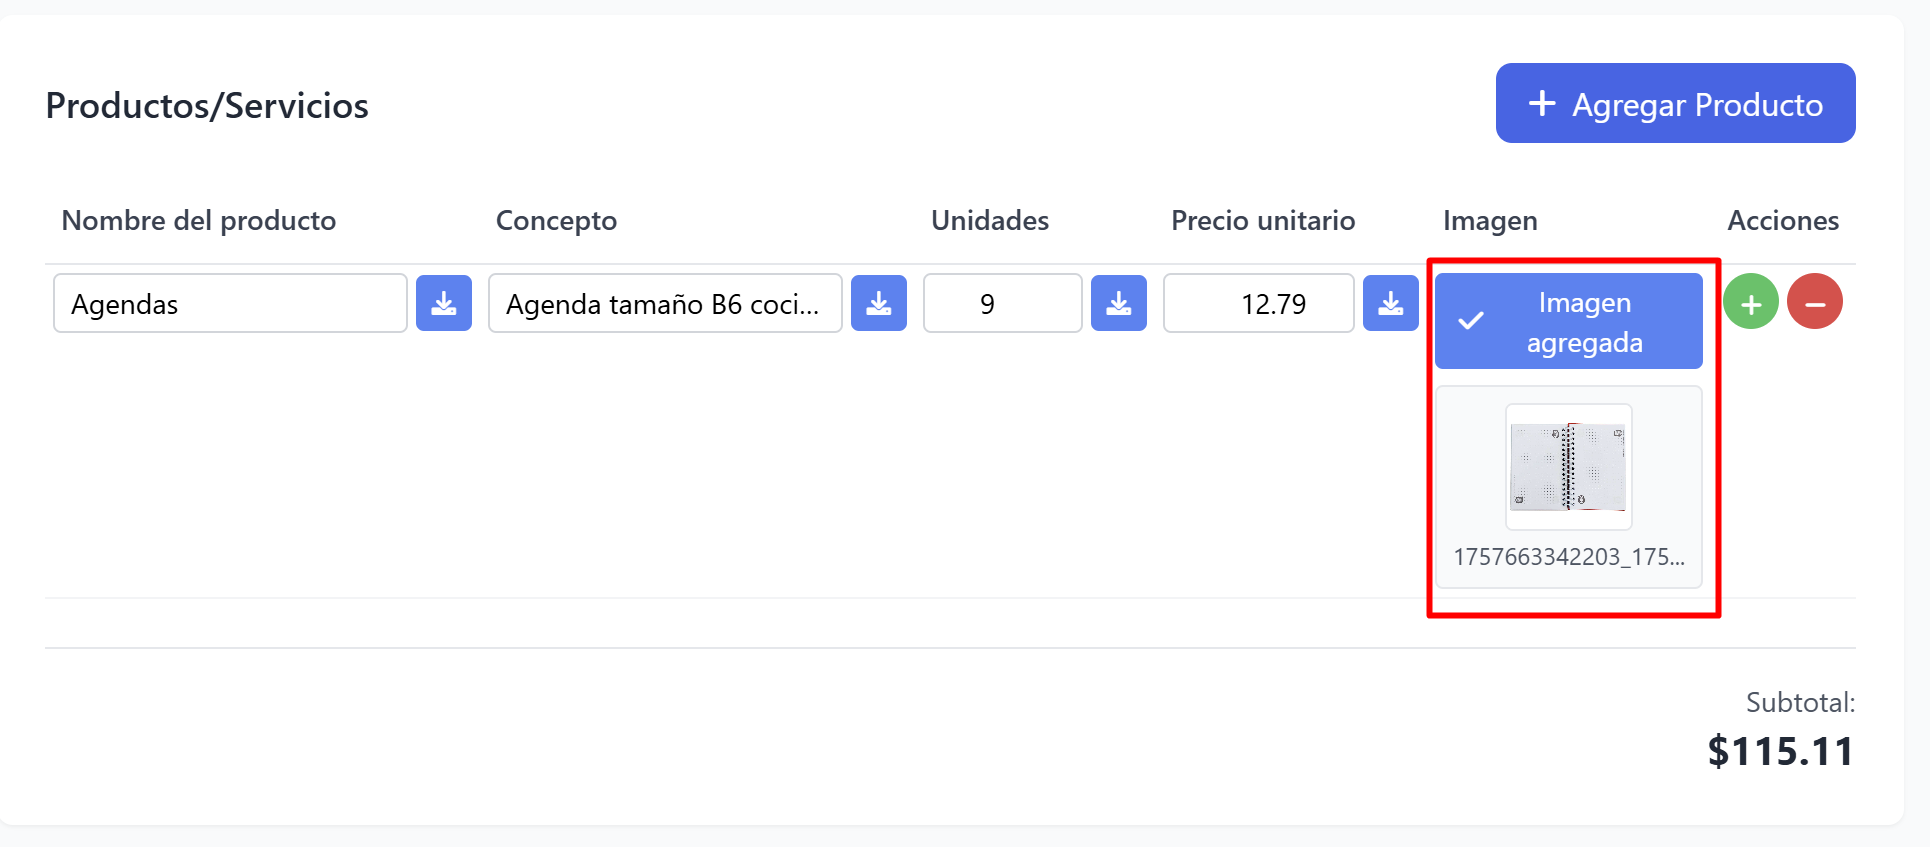
\includegraphics[width=0.8\linewidth]{img/imagen_agregada.png}
    \caption{Vista previa de la imagen agregada a un producto o servicio.}
    \label{fig:imagen_agregada}
\end{figure}
Si deseas cambiar la imagen, simplemente haz clic en el botón azul \textbf{Imagen agregada} que se encuentra arriba de la imagen, se 
abrirá nuevamente el Explorador de archivos y podrás seleccionar una nueva imagen para reemplazar la anterior.
\begin{importante}[Nota importante]
No es necesario agregar una imagen a cada producto o servicio. Si no deseas agregar una imagen, simplemente deja el campo vacío.
\end{importante}

\begin{minipage}{0.78\linewidth}
    Para cada producto que se agregue a la tabla, en la última columna aparecerán dos botones de acciones
    (figura \ref{fig:icono_acciones}). El primer botón, con el ícono de un '+' permite crear una nueva
    fila con campos vacíos para registrar un nuevo producto. El segundo botón es un signo menos, que sirve 
    para borrar el registro de producto.
\end{minipage}
\hfil   
\begin{minipage}{0.08\linewidth}
    \begin{figure}[H]
        \centering
        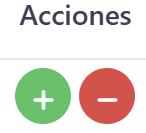
\includegraphics[width=0.99\textwidth]{img/boton_acciones.png}
        \caption{}
        \label{fig:icono_acciones}
    \end{figure}
\end{minipage}
\vspace{0.5cm}
\\Cuando hayas terminado de agregar todos los productos o servicios, puedes proceder a guardar la cotización
 siguiendo el mismo procedimiento descrito anteriormente. No cambies de página sin antes haber guardado la cotización.
\subsection{Cómo editar una cotización}
Para editar una cotización existente, dirígete a la página de \textbf{Cotizaciones guardadas} donde se muestra la tabla con todas las cotizaciones previamente registradas, luego
    ubica la cotización que deseas editar y haz clic en el botón \textbf{Editar} que se encuentra en la columna de acciones, como se muestra en la figura~\ref{fig:editar_cotizacion}.
\begin{figure}[H]
    \centering
        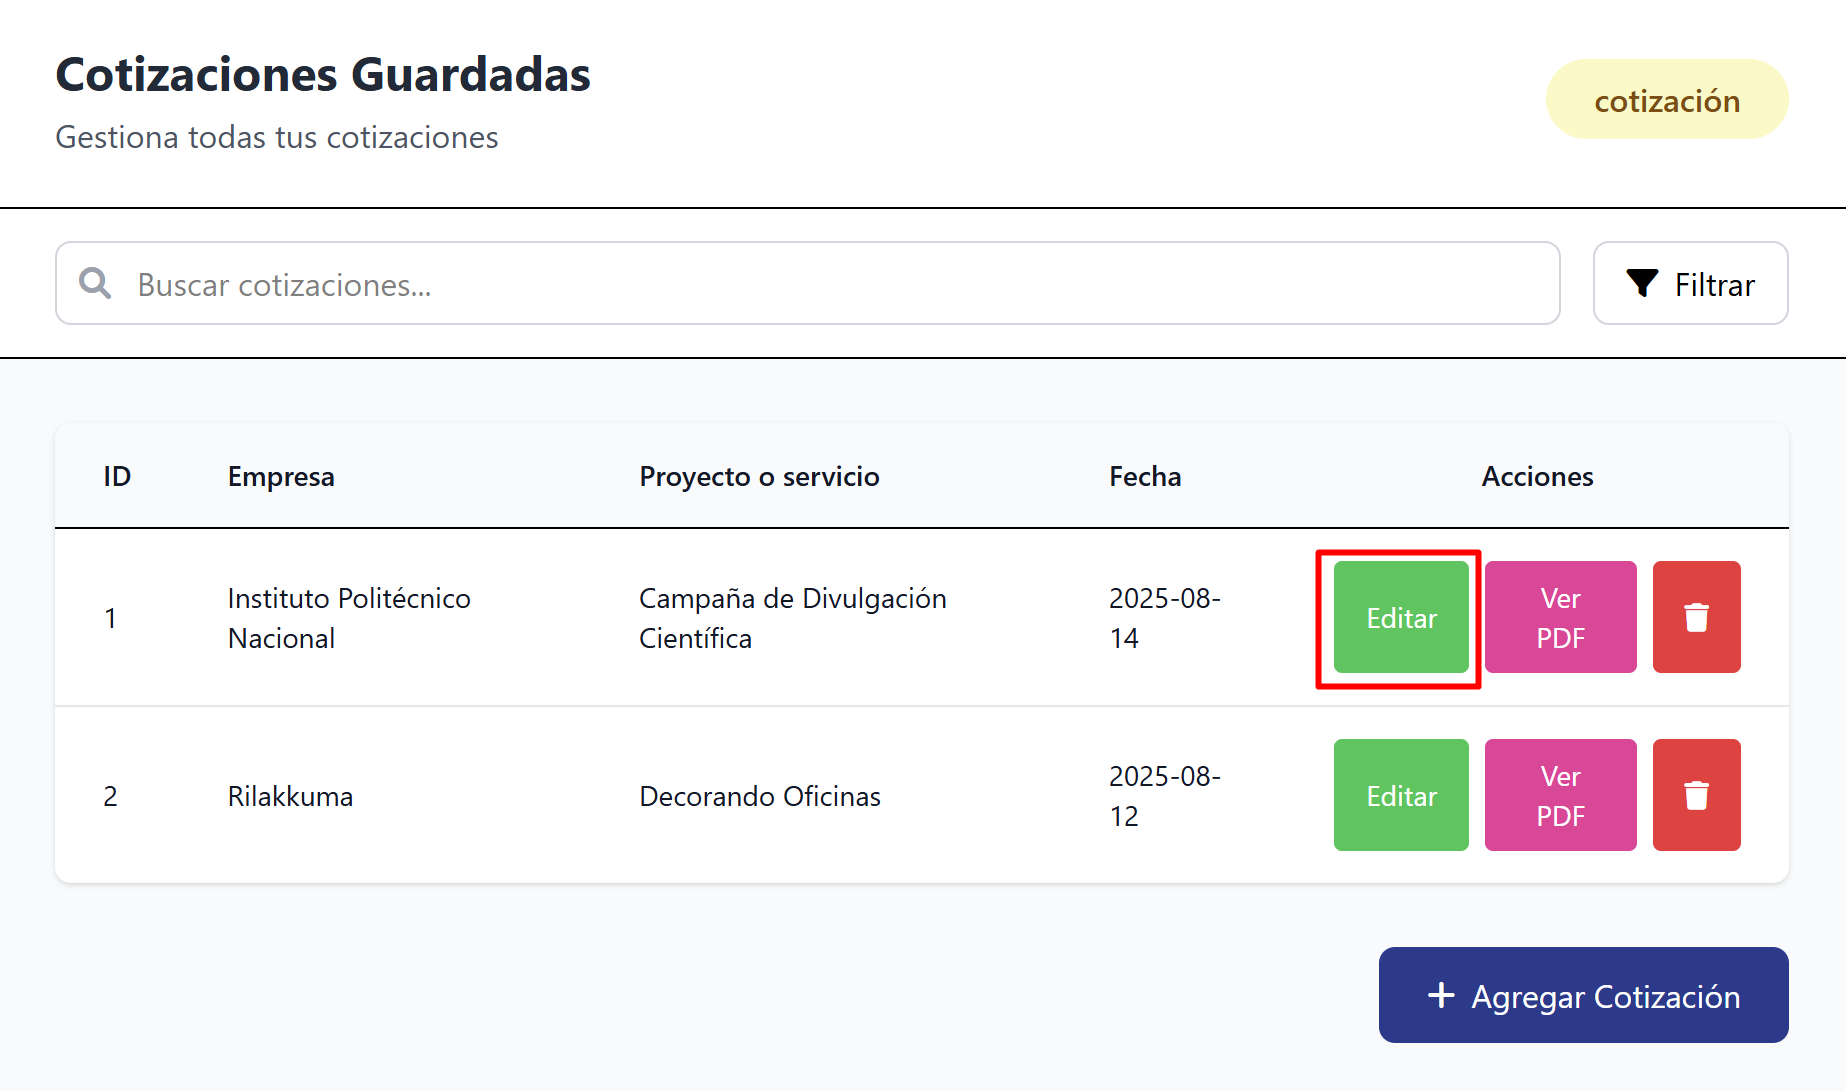
\includegraphics[width=0.8\linewidth]{img/editar_cotizacion.png}
    \caption{Botón para editar una cotización existente.}
    \label{fig:editar_cotizacion}
\end{figure}
Esto te llevará a la página de agregar cotización, pero esta vez, los campos estarán llenos con la información de la cotización seleccionada.
Realiza los cambios necesarios en los campos correspondientes. Puedes modificar cualquier detalle de la cotización, incluyendo los productos o servicios, cantidades, precios, quitar la imagen
de un producto, abrir un nuevo documento de Excel, etc.
\begin{figure}[H]
    \centering
        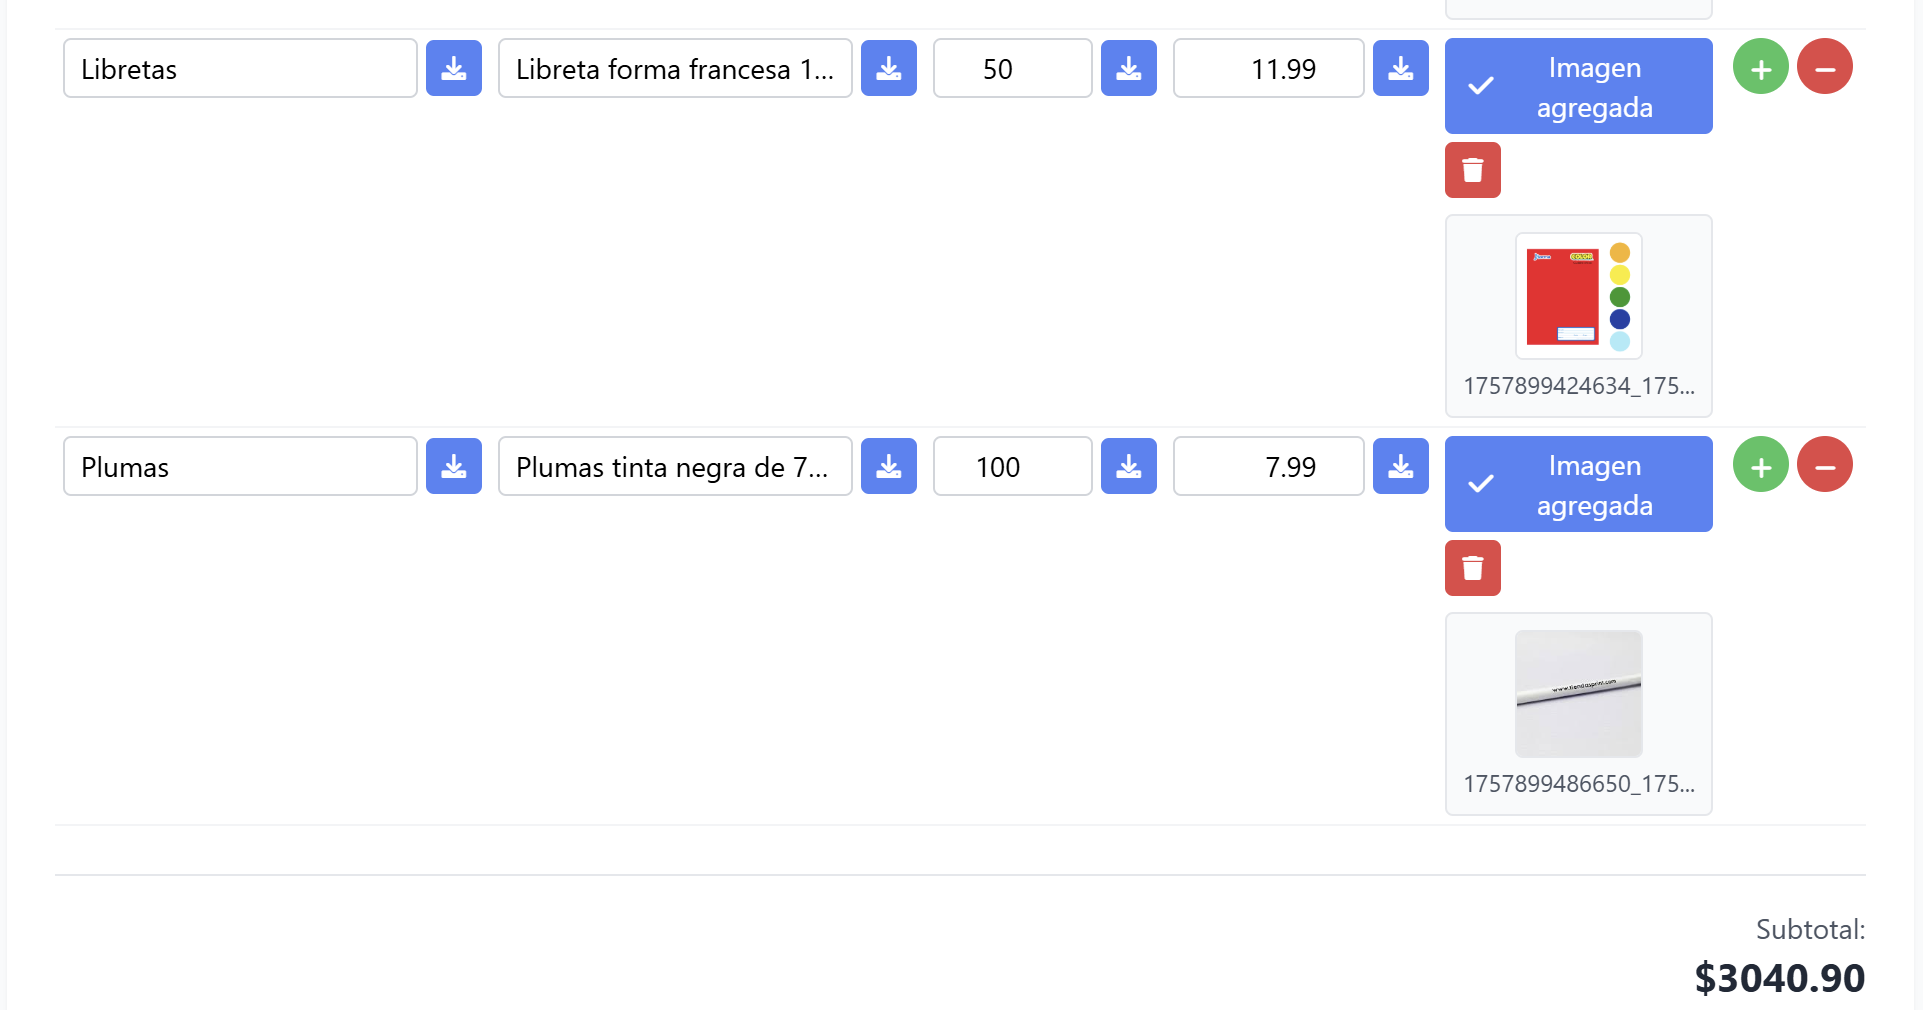
\includegraphics[width=0.8\linewidth]{img/editar_producto.png}
    \caption{Los campos estarán llenos con la información de la cotización seleccionada, da clic en los campos para editarlos.}
    \label{fig:editar_producto}
\end{figure}
Una vez que hayas realizado los cambios, asegúrate de guardar la cotización nuevamente haciendo clic en el botón \textbf{Actualizar Cotización}. 
Si todos los campos obligatorios están completos, la cotización se guardará correctamente y serás redirigido de vuelta a la página de \textbf{Cotizaciones guardadas}.
\subsection{Cómo eliminar una cotización}
Dirígete a la página de \textbf{Cotizaciones guardadas} y ubica la cotización que deseas eliminar. Haz clic en el botón rojo que contiene un icono de un bote de basura,
 se encuentra en la columna de acciones, como se muestra en la figura~\ref{fig:eliminar_cotizacion}. 
\begin{figure}[H]
    \centering
        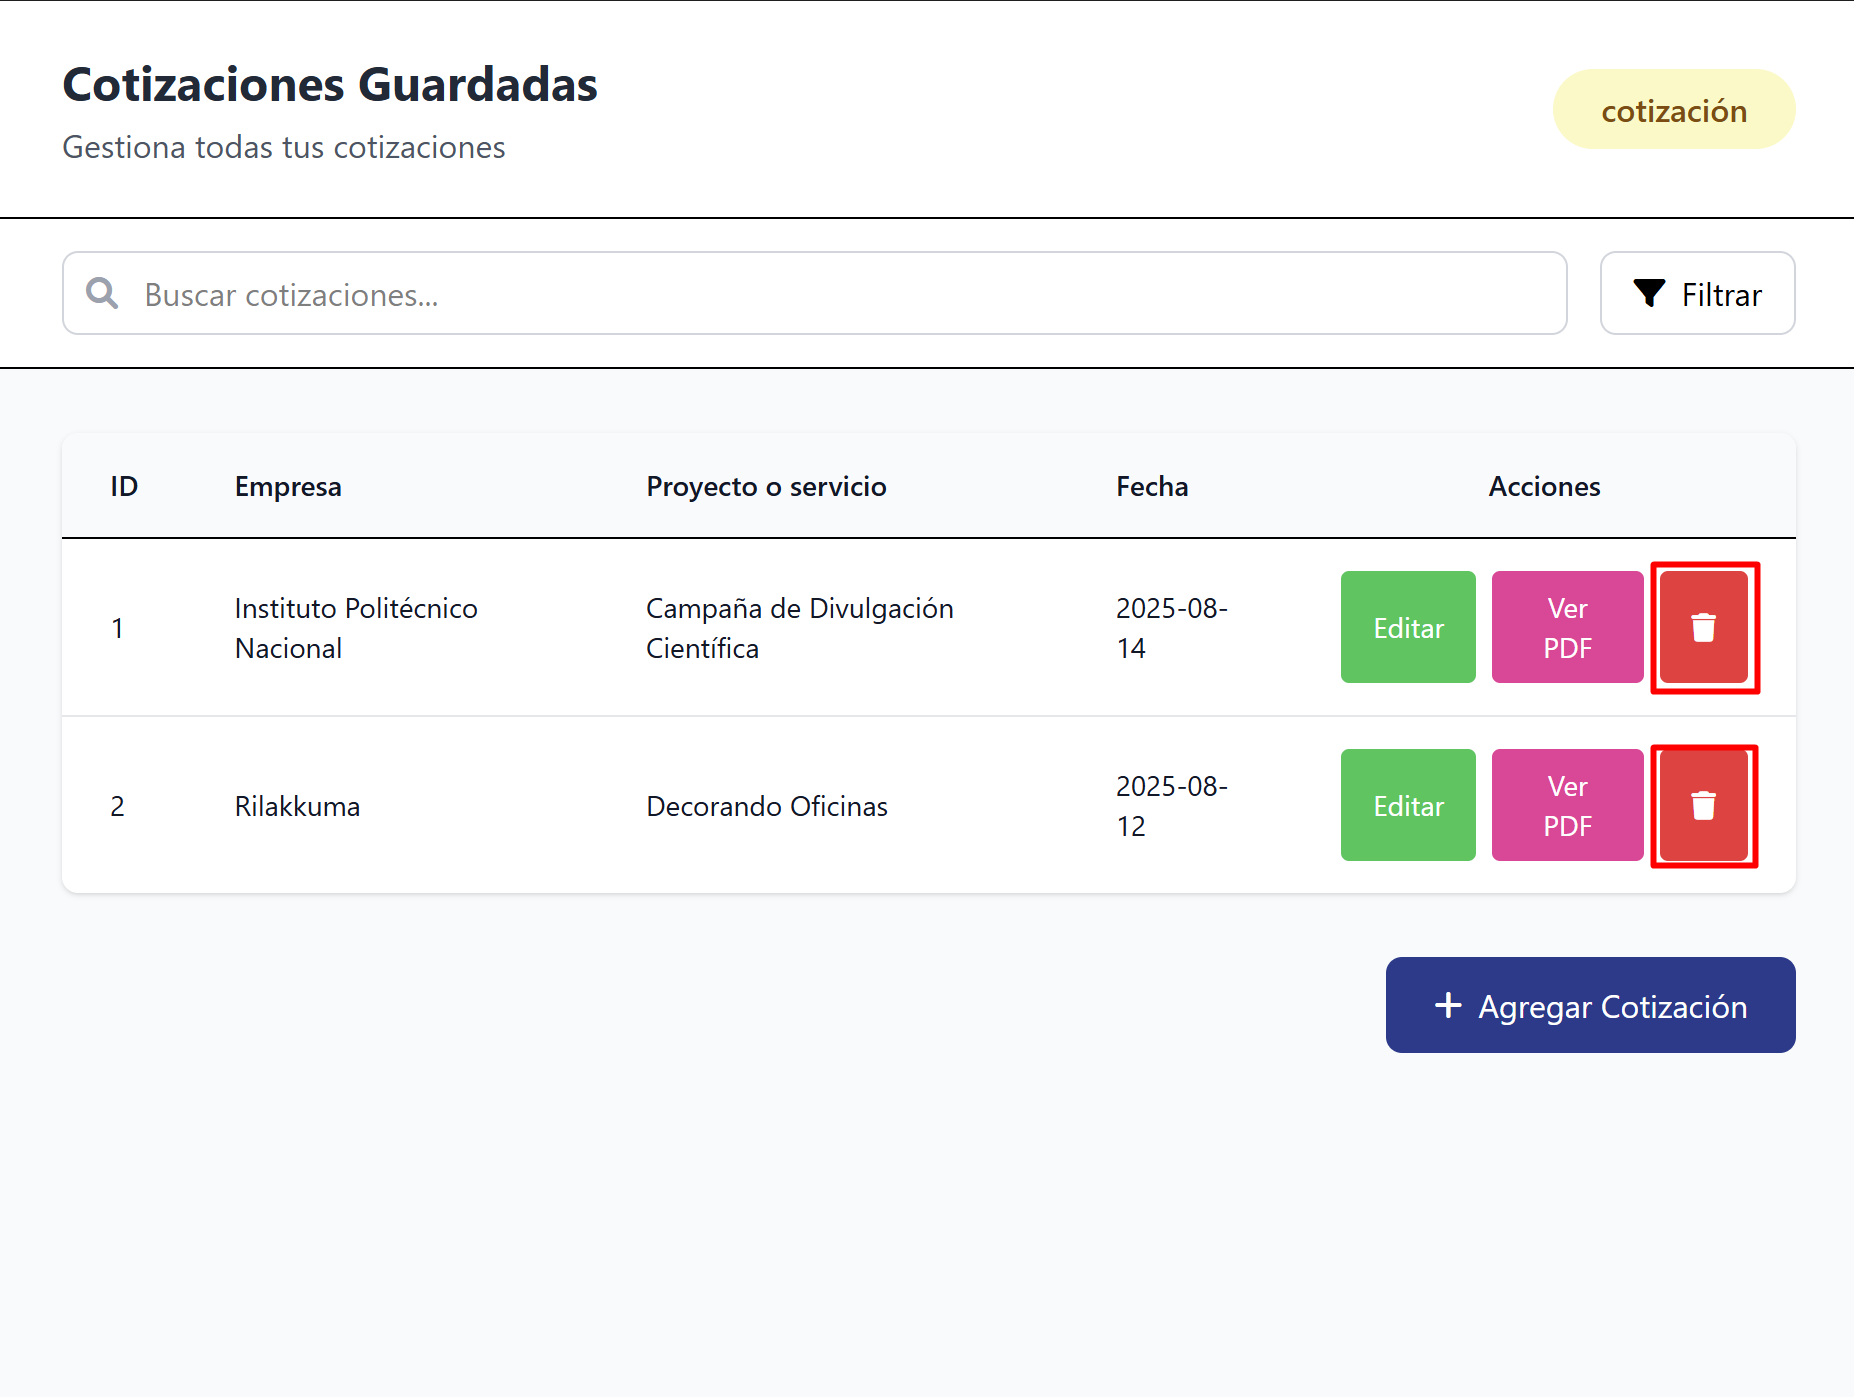
\includegraphics[width=0.8\linewidth]{img/eliminar_cotizacion.png} 
    \caption{Botón para eliminar una cotización existente.}
    \label{fig:eliminar_cotizacion}
\end{figure}
 Un cuadro de diálogo aparecerá verificando que efectivamente desea borrar la cotización, si está seguro, haga clic en \textbf{Eliminar}, de lo contrario, 
 seleccione \textbf{Cancelar} para cancelar la acción. Si decide eliminar el registro, esta será borrado permanentemente y ya no podrá recuperarse.
\begin{figure}[H]
    \centering
        \fbox{
            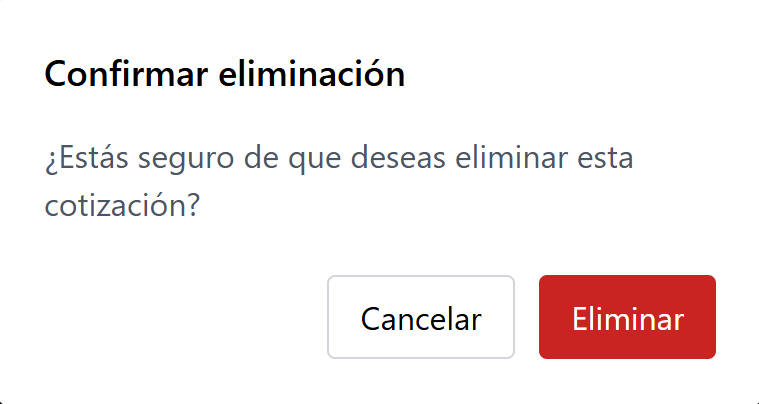
\includegraphics[width=0.4\linewidth]{img/mensaje_confirmacion.png}
        }
    \caption{Cuadro de diálogo para confirmar la eliminación de una cotización.}
    \label{fig:cuadro_eliminar}
\end{figure}
\subsection{Generación del PDF de la cotización}
Para generar el archivo PDF de una cotización, dirígete a la página de \textbf{Cotizaciones guardadas} y ubica la cotización de la cual deseas generar el PDF.
Haz clic en el botón \textbf{Ver PDF} que se encuentra en la columna de acciones, como se muestra en la figura~\ref{fig:generar_pdf}.
\begin{figure}[H]
    \centering
        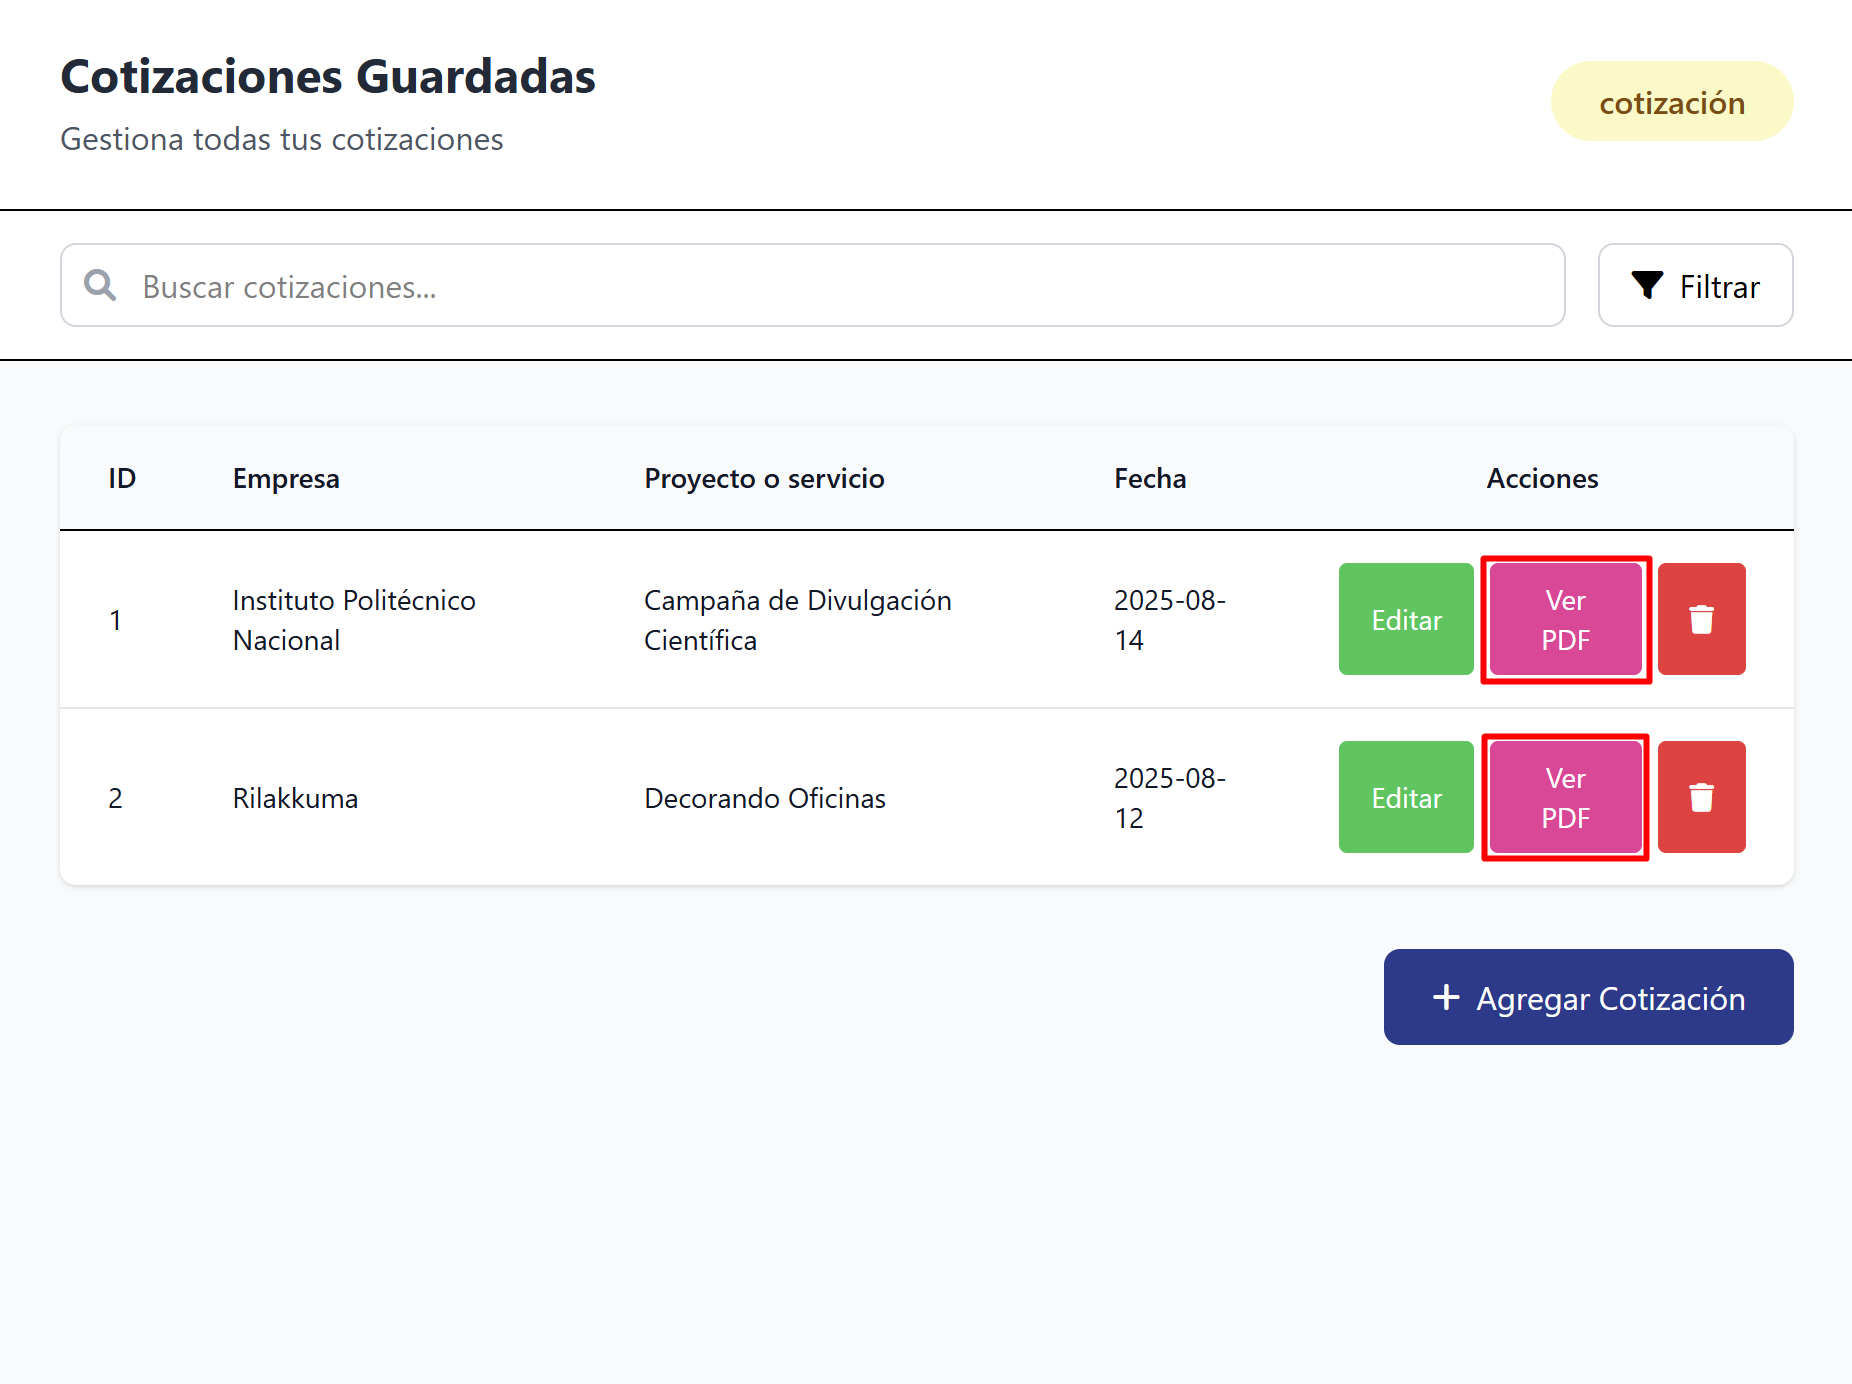
\includegraphics[width=0.8\linewidth]{img/generar_pdf.png}
    \caption{Botón para generar el archivo PDF de una cotización existente.}
    \label{fig:generar_pdf}
\end{figure}
Aparecerá un mensaje de cargando y cuando el pdf esté listo, se abrirá automáticamente en el lector de PDF predeterminado de tu sistema. 
\begin{figure}[H]
    \centering
        \fbox{
            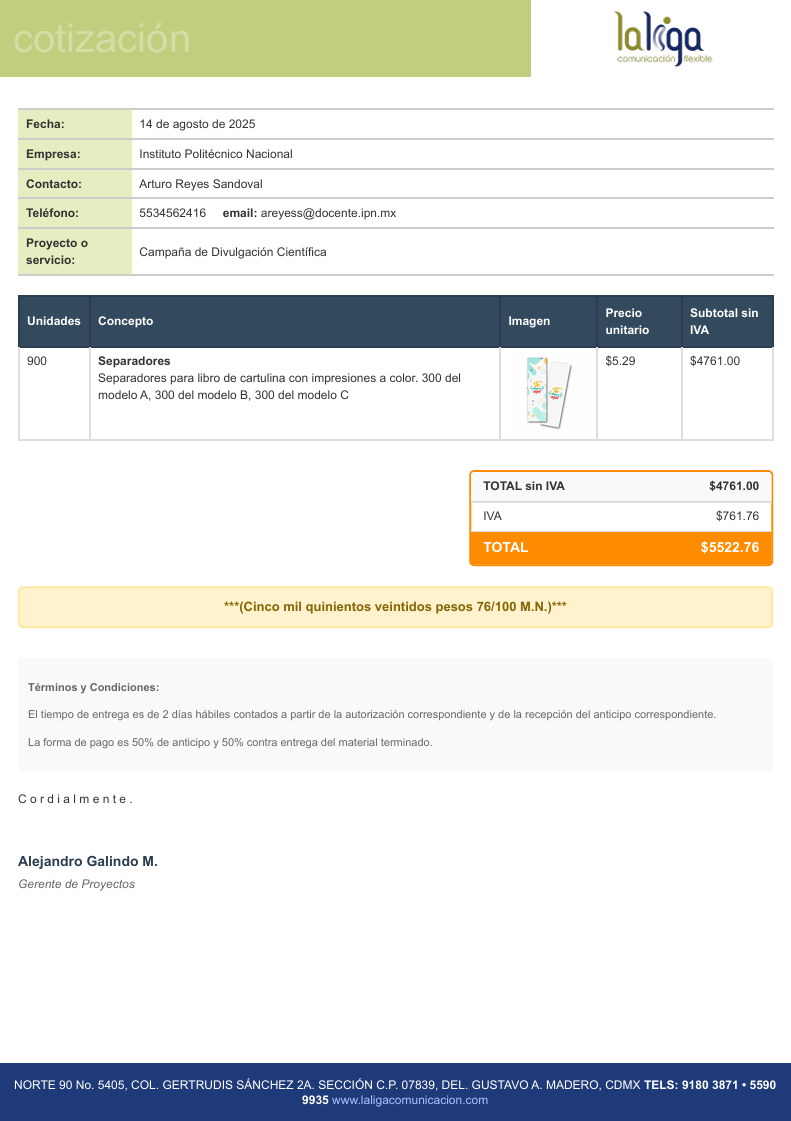
\includegraphics[width=0.4\linewidth]{img/resultado_pdf.png}
        }
    \caption{Ejemplo de pdf generado a partir de un registro.}
    \label{fig:resultado_pdf}
\end{figure}
%%%%%%%%%%%%%%%%%%%%%%%%%%%%%%%%%%%%%%%%%%%%%%%%%%%%
\section{Resolución a problemas comunes}
\begin{definicion}[No abre correctamente el archivo excel]
    En caso de que no abra correctamente el archivo excel, asegúrese de que el archivo esté en formato .xlsx y que la hoja seleccionada contenga datos válidos. Verifique también que el archivo no esté protegido con contraseña.
\end{definicion}
\vspace{0.7cm}
\begin{definicion}[Error al generar el PDF]
    Asegurate de que todos los campos obligatorios esten completos y que haya errores en los datos ingresados. Si el problema persiste, intente reiniciar la aplicación y volver a generar el PDF.

\end{definicion}
\vspace{0.7cm}
\begin{definicion}[No se muestran las imágenes]
    
Asegúrese de que las imágenes estén en el formato correcto (JPEG, PNG) y que la ruta del archivo sea válida. Verifique también que las imágenes no estén dañadas.
\end{definicion}
\vspace{0.7cm}
\begin{definicion}[Problemas al ingresar datos]
    Este puede ser un error comun en la aplicacion, en caso de que no se pueda ingresar algun campo, cambie a otra aplicacion y vuelva a la aplicacion de cotizaciones, esto deberia solucionar el problema.
\end{definicion}

\begin{definicion}[Error: A Javascript error occurred in the main process]
    Si al estar registrando una cotización aparece una ventana como la de la figura~\ref{fig:error}, solo cierre el cuadro de diálogo
    dando clic sobre el botón 'ok', este errror no es grave e indica que hay campos que se dejaron vacíos.
    \begin{figure}[H]
        \centering
        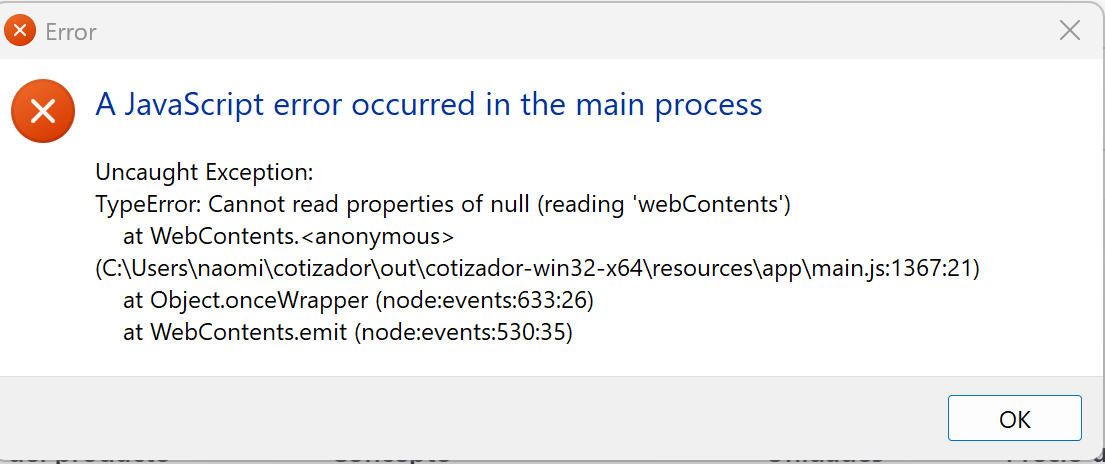
\includegraphics[width=0.99\textwidth]{img/error.png}
        \caption{}
        \label{fig:error}
    \end{figure}
\end{definicion}


\subsection{Soporte y contacto}

Para aistencia adicional, puedes contactar al soporte técnico a través del correo electrónico: aaronugaldet@gmail.com
\pagebreak

\end{document}